\chapter{Enzyme Kinetics}
\label{chap:enzyme-kinetics}

{\bf Enzyme kinetics} is the study of chemical reactions in which substrate 
are catalyzed by an enzyme. In such reactions, the process is quite
complicated and thus, often divided into a number of elementary
reaction~\footnote{\url{http://en.wikipedia.org/wiki/Enzyme_kinetics}} which
contains fast reactions and slow reactions.

Although the law of mass action has been widely used to explain reversible
chemical reactions (Sect.\ref{sec:law-mass-action}), it is typically impossible
to apply that to chemical reactions that involve enzyme, unless multiple steps
are used. \textcolor{red}{However, in enzyme kinetics, there are
situations that the law
  of mass action is invalid: (1) at high concentration, doubling the
  concentration of one reactant need not double the overall reaction; (2) at
  extremely low concentration, it may not be appropriate to represent
  concentration as a continuous variable}.

\section{Introduction}

The enzyme usually manipulate other molecules - the {\it substrate} -
by allowing the substrate to bind to the enzyme's
active site; thus allow the substrate to be transformed into products
through a series of steps known as {\it enzymatic mechanism}, as shown
in Fig.~\ref{fig:enzyme_subs}. 

{\it In vivo}, the enzyme activity can be exerted by
\begin{enumerate}
  \item binding to small molecules: substrates or effectors (inhibitors,
  and activators), at catalytic or regulatory sites on the enzymes

  \item modification the enzyme through either covalent changes
  (hydrolysis, phosphorylation, ...), or noncovalent changes
  (polymerization/depolymerization, ...)
\end{enumerate}
In general, an enzyme can bind to a single substrate or multiple substrates.
Although this mechanism is often going through a complex series of steps, the
rate of the overall process is determined by the step that is slowest. This {\it
rate-determining step} can be a chemical reaction or a conformational change of
the enzyme or substrate(s). It is similar to the rate-limiting step in
multi-step chemical reaction (Sect.\ref{sec:multiple-step-reaction}).


\begin{figure}[hbt]
 \centerline{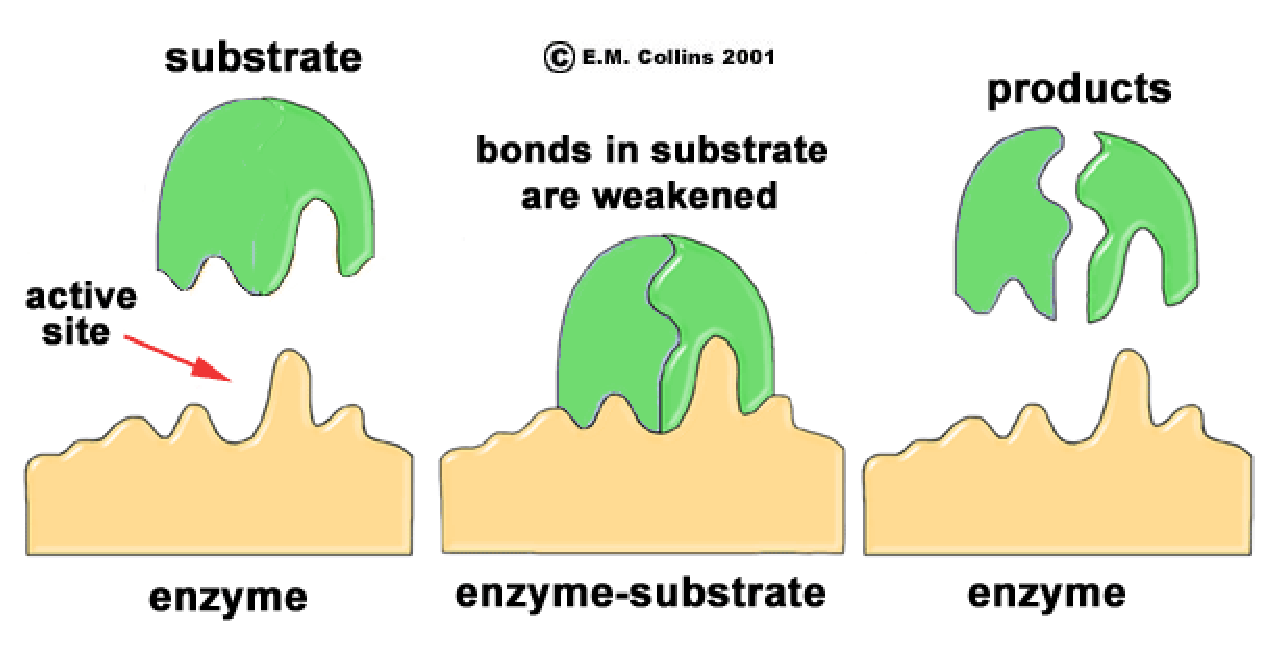
\includegraphics[height=4cm]{./images/enzyme_substrate.eps}}
\caption{Enzyme mechanism}
\label{fig:enzyme_subs}
\end{figure}


{\bf Example}: Consider this chemical reactions: enzymes $E$ help
accelerate the conversion from the substrate $S$ into the product
$P$. Enzyme reaction does not follow the law of mass action, as the
rate of the reaction (catalysis) does not show a linear response to an
increasing substrates, i.e. the rate of the reaction vs. the substrate
concentration is a hyperbolic curve, as shown in
Fig.~\ref{fig:rate_reaction}.

\begin{figure}[hbt]
 \centerline{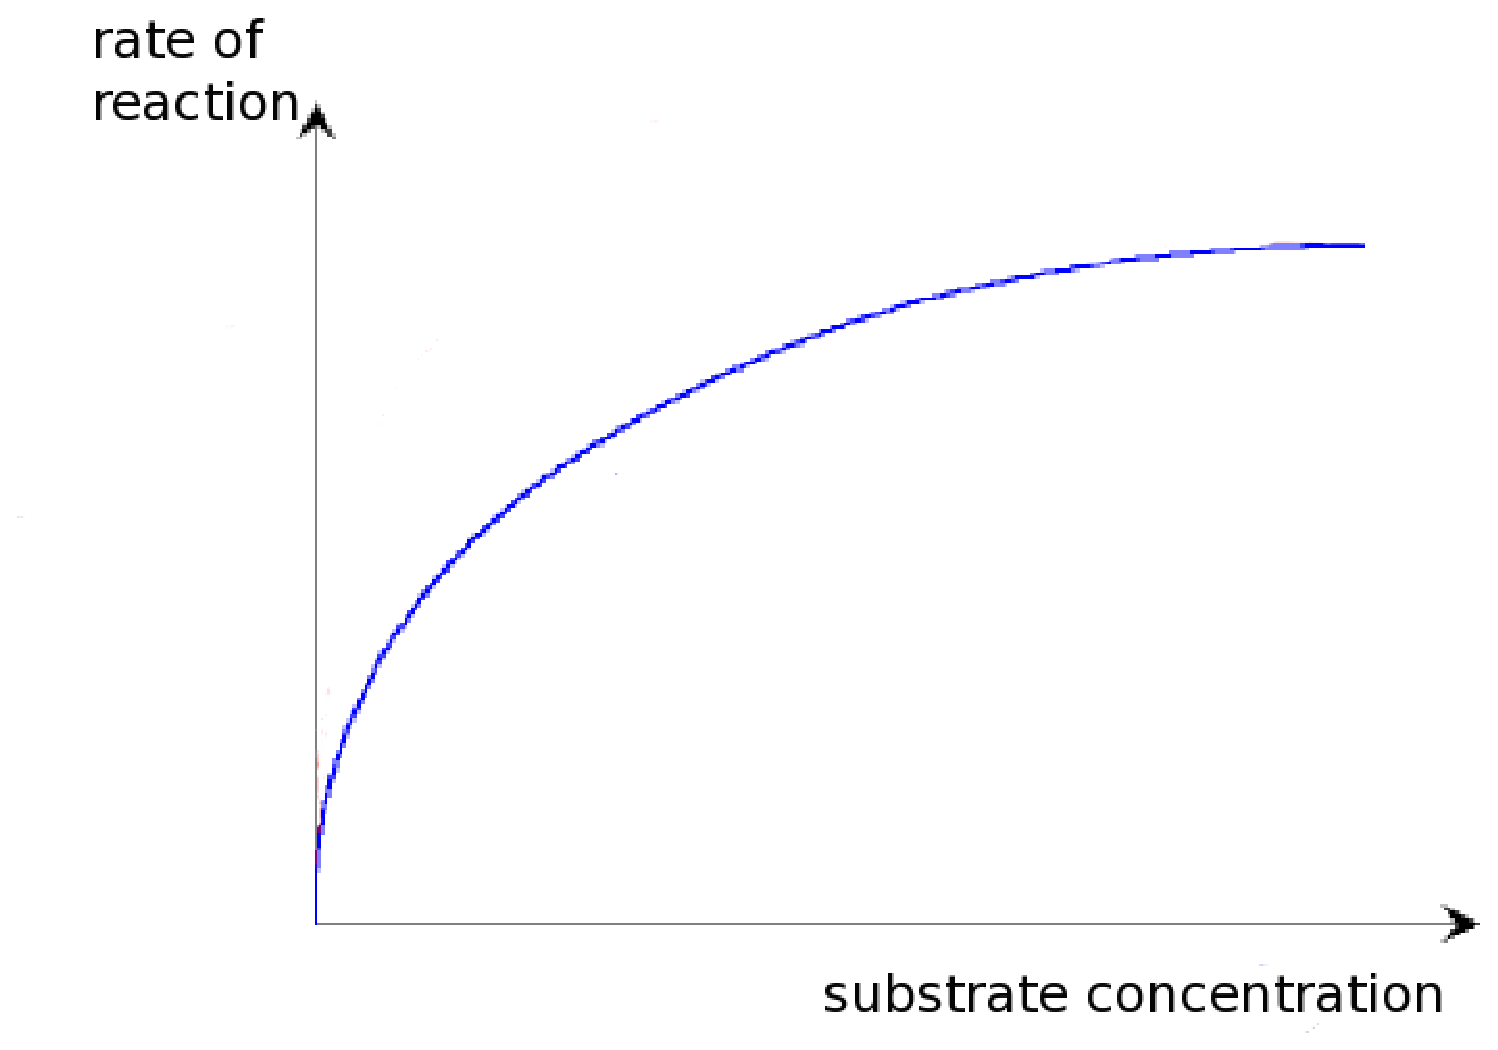
\includegraphics[height=5cm]{./images/rate_reaction.eps}}
 \caption{Rate of reaction}
 \label{fig:rate_reaction}
\end{figure}


In enzyme kinetics, there are two major approaches: the classical {\it
deterministic} approach (Sect.\ref{sec:enzyme-kinetics-deterministic}), and the
modern {\it stochastic} approach (Sect.~\ref{sec:stoch-model-enzyme}). However,
a major challenge when solving a system of multiples reactions is that the time
step is contrained by the fastest reaction, i.e. smallest {\it time constant}.


\section{One-binding site approach}
\label{sec:enzyme-kinetics-deterministic}

The one-binding site model is used when the velocity of product formation
follows the hyperbolic curve, Fig.\ref{fig:hyperbolic_sigmoidal_relationship}.
Michaelis-Menten kinetics (Sect.\ref{sec:equil-appr}) requires 2
assumptions\footnote{\url{http://depts.washington.edu/wmatkins/kinetics/quadratic.html}}:
\begin{enumerate}
\item free ligand (substrate) approximation [S]$\approx s_0$

[S] is close to the total substrate concentration in the system $s_0$ which is
the true independent variable in most experimental set-ups. This is valid when
the amount of substrate is much higher than the amount of enzyme

\item rapid equilibrium (of the substrate), $d[S]/dt=0$
\end{enumerate}
% \item steady-state approximation (of the complex), $d[ES]/dt=0$

The Briggs-Haldane modification for Michaelis-Menten kinetics
(Sect.\ref{sec:quasi-steady-state}) replaces the second assumption with
steady-state approximation $d[ES]/dt\approx 0$. 

Morrison kinetics remove also the first assumption
(Sect.\ref{sec:morrison-kinetics}).

If the binding site at the enzyme can be bound by a molecule other the
substrate, and thins binding inhibit the binding of the substrate, the need to
use a competitive one-site model (Sect.~\ref{sec:competitive-one-site}).

\subsection{One-site model}
\label{sec:mich-ment-kinet}

To explain the conversion of the substrate $S$ to product $P$ by enzyme $E$,
Michaelis-Menten in 1913 proposed a model that is now considered as a classical
deterministic theory of enzyme kinetics \citep{michaelis1913kir}.

They postulated that at first $E$ bind to $S$ forming a complex, denoted by $ES$
(some use the notation $C$), which then either (1) separate or (2) breaks down
into the product $P$ and releasing $E$.

\begin{eqnarray}
  \label{eq:261}
  \left\{  
    \begin{array}{lcc}
      \ce{E + S ->[k_1] ES} & \text{association} & \text{(rapid)} \\
      \ce{ES ->[k_2] E + S} & \text{dissociation} & \text{(rapid)} \\
      \ce{ES ->[k_3] E + P} & \text{decomposition} & \text{(slow)}
    \end{array}
\right.
\end{eqnarray}
with $k_i$ are deterministic rate constants. Remember in
Sect.\ref{sec:elementary-reactions}, the unit of $k_2,k_3$ are sec$^{-1}$, while
that of $k_1$ is M$^{-1}$.sec$^{-1}$.

At individual step,the law of mass action is applied to each reaction and
yields 4 differential equations for the rate of change of [S], [E], [P], [ES].
NOTE: The power term for each concentration is 1 as this is elementary
reaction.

\begin{equation}
  \label{eq:267}
  \begin{split}
    % \frac{d[S]}{dt} &= k_{-1}[ES] - k_1[S][E] \\
    % \frac{d[E]}{dt} &= k_{-1}[ES] - k_1[S][E] + k_2[ES] \\
    % \frac{d[ES]}{dt} &= -k_{-1}[ES] + k_1[S][E]  - k_2[ES] \\
    % \frac{d[P]}{dt} &= k_2[ES]
    \frac{d[S]}{dt} &= k_{2}[ES] - k_1[S][E] \\
    \frac{d[E]}{dt} &= k_{2}[ES] - k_1[S][E] + k_3[ES] \\
    \frac{d[ES]}{dt} &= -k_{2}[ES] + k_1[S][E]  - k_3[ES] \\
    \frac{d[P]}{dt} &= k_3[ES]
  \end{split}
\end{equation}

Due to the two conservation laws: total amount of enzyme is
preserved, and total amount of substrate is preserved.
\begin{equation}
  \label{eq:279}
  \begin{split}
      [E] + [ES] &= E_T = e_0 \\
      [S] + [ES] + [P] &= s_0
  \end{split}
\end{equation}
The four ODEs can be reduced to two
\begin{equation}
  \label{eq:280}
  \begin{split}
    % \frac{d[S]}{dt} &= k_{-1}(e_0-[E]) - k_1[S][E] \\
    % \frac{d[E]}{dt} &= (k_{-1}+k_2)(e_0-[E]) - k_1[S][E]  \\
    \frac{d[S]}{dt} &= k_{2}(e_0-[E]) - k_1[S][E] \\
    \frac{d[ES]}{dt} &= -(k_{2}+k_3)[ES] + k_1[S](e_0-[ES])
    % \frac{d[E]}{dt} &= (k_{2}+k_3)(e_0-[E]) - k_1[S][E]  \\
  \end{split}
\end{equation}
with initial condition $(s_0, e_0)$. How can we solve this set of ODEs
since they can not be integrated explicitly. Let's look at different
hypothesis in the coming sections.




\subsection[Michaelis-Menten assumption]{Michaelis-Menten assumption:
equilibrium approximation of substrate [S]}
\label{sec:equil-appr}
\label{sec:Michaelis-Menten-formula}

To be able to solve eq.~\eqref{eq:280}, Michaelis and Menten
\textcolor{red}{assumed that the enzyme concentration is much less than the
substrate concentration}, i.e. $e_0 < s_0$. So, at equilibrium, 
the substrate concentration doesn't change,
e.g. $d[S]/dt=0$, or
\begin{equation}
  \label{eq:281}
  \frac{[S][E]}{[ES]} = \frac{k_{2}}{k_1}
\end{equation}
% This is known as the equilibrium assumption, i.e. the association and
% diassociation of the substrate to the enzyme is 

It means that 
\textcolor{red}{the rate of decomposition is slow enough so that it
  doesn't disturb the association-disassociation equilibrium}
( $k_{2} \gg k_3$).  Thus, it allows the association-disassociation
steps to be treated as an isolated system $\ce{A <=> B}$.  In other
words, a compact form is
\begin{eqnarray}
  \label{eq:263-c}
    \left\{  
    \begin{array}{lcc}
      \ce{E + S <=>[k_1][k_2] ES} & \text{association/diassociation} & \text{(rapid)} \\
      \ce{ES ->[k_3] E + P} & \text{decomposition} & \text{(slow)}
    \end{array}
\right.
\end{eqnarray}
% or
% \begin{equation}
%   \label{eq:266}
% %  S + E \ce{<=>[k_1][k_{-1}]} C \ce{->[k_2]} P + E
%   S + E \ce{<=>[k_1][k_{2}]} C \ce{->[k_3]} P + E
% \end{equation}
% or
% \begin{equation}
%   \label{eq:289}
%    S + E \ce{<=>[k_1][k_{2}]} ES \ce{->[k_3]} P + E
% \end{equation}

%  it is
% supplied by a reservoir or the change is negligible. Thus, it is at
% equilibrium with the complex swiftly, or
% and

Noting that [E]+[ES] = $e_o$ with $e_o$ is the initial concentration of $E$,
then
\begin{equation}
  \label{eq:295}
      % [ES] &= \frac{k_1}{k_{-1}}[S](e_0-[ES]) \\
     [ES] = \frac{k_1}{k_{2}}[S](e_0-[ES]) 
\end{equation}
or
\begin{equation}
  \label{eq:296}
      % [ES] = \frac{e_0[S]}{\frac{k_{-1}}{k_{1}}+[S]} 
      [ES] = \frac{e_0[S]}{\frac{k_{2}}{k_{1}}+[S]} 
\end{equation}
or, from eq.~\eqref{eq:295}, the rate of product formation is
\begin{eqnarray}
  \label{eq:1}
  v = \frac{d[P]}{dt} = k_3 \ce{[ES]} =  k_3e_0\frac{[S]}{K_m+[S]} 
\end{eqnarray}
with $K_d=\frac{k_2}{k_{1}}$ is the dissociation constant and has the unit as
concentration, i.e. M (molar), mM (milimolar, or milimoles per litre or mmoles
per litre).  

As we can see in eq.~\eqref{eq:1}, due to the fast kinetics of the ES complex
formation, the rate of forming the product P is  determined by $k_3$.

If we assign $v_\max = k_3 e_0$, then
the rate of product creation is 
\begin{equation}
  \label{eq:310}
  v = v_\max \frac{[S]}{K_m+[S]}
\end{equation}
with [S] is usually assumed to be equal to the initial concentration
of substrate $s_0$. The unit of $v_\max$
is the same as that of $v$, i.e. [mM/sec].

\begin{framed}
  The value of $v_\max$ represents the \textcolor{red}{maximum velocity
  achieved by the system, and this happens when the substrate is so ``abundant'',
  i.e. very ``high'' concentration of [S]}. The exact of 'abundant' is dependent
  on the type of substrate, some substrate reaches the maximum speed at quite
  low concentration, and if we add more, it doesn't change the reaction
  velocity.

  $K_m$ (sometimes represented as $K_S$) represents the
  \textcolor{red}{concentration of substrate at which the reaction velocity
  reaches 50\%  of $v_\max$}.
%   So, aka half-maximal constant as it is the concentration of substrate at which
%   half of the reaction has occurred.
  The meaning of $K_m$ is related to the affinity of the substrate for
the enzyme. If $K_m$ has very low concentration in relative to the resting
level of [S] then substrate has a high affinity for the enzyme.
   
\end{framed}

{\bf SUMMARY}: In summary, Michaelis-Menten equation describes how the
reaction rate $rate$ depends on the positions of the substrate-binding
equilibrium and the rate constant $k_3$.
\textcolor{red}{However, there is the contrary: if [S] doesn't change,
  then S would not be used up, i.e. S must be of very huge amount of
  there must be a large reservoir supplying S?}.
In practice, this is not realistic, especially {\it in vivo}.  This
pointed out that eq.~\eqref{eq:263-c} is not a good approximation.  


% This lead to the
% classical {\it hyperbolic Michaelis-Menten equation}, as shown in
% Fig.~\ref{fig:rate_reaction}, relating the rate of forming $P$ to the
% concentration of the substrate $S$ (to be explained shortly).
% \begin{eqnarray}
%   \label{eq:262}
%   v = v_\max\frac{[S]}{\frac{k_2}{k_1}+[S]}
% \end{eqnarray}
% with $V=k_3E_T$ (given $E_T=[E]+[ES]$), the total enzyme concentration
% in the complex). 

\subsection[Briggs-Haldane assumption]{Briggs-Haldane assumption: quasi- (or
pseudo-) steady-state approximation of complex [ES]}
\label{sec:quasi-steady-state}
\label{sec:Michaelis-Menten-modified}

The steady-state assumption of Michaelis and Menten was somehow unrealistic as
their assumption means there is no change in S. 

To resolve that problem, instead of using steady-state assumption, Bridges and
Haldane (1925)~\citep{briggs1925nke} used a quasi-steady state equilibrium for
ES. It means that ES both involves in fast and slow process, yet the net
concentration doesn't change.

Still using the assumption that \textcolor{red}{the enzyme concentration is much
less than the substrate concentration}, i.e. $s_0\gg e_0$.
This is logical because the enzyme only need a small concentrations compared to
that of the substrate for the reaction to occur~\citep{li2008qssa}, e.g.
$\epsilon = \frac{e_0}{s_0}$ is typical in the range $10^{-2}$ to $10^{-7}$.


The new interpretation is
\begin{equation}
  \label{eq:289}
  S + E \ce{<=>[k_1][k_{2}]} ES \ce{->[k_3]} P + E
\end{equation}


  Under the above assumption, soon after the beginning of the
  reaction, the concentration of the complex ES reaches its
  steady-value. This transient occur so fast as to be unobservable. It
  means that after the complex is ``filling up'', its concentration
  changes much more slower than those of the product [P] and substrate
  [S]. Thus, it can be considered that [ES] was essentially doesn't
  change over time, i.e. $d[ES]/dt\approx 0$ rather than using
  $d[S]/dt=0$. 

In essence, the complex is assumed to be in    {\it quasi-steady-state
assumption} (QSSA) (or pseudo-steady-state)  and the overall rate of reaction is
determined solely by $k_2$ (the rate is  generally orders of magnitude lower
than $k_1$)\footnote{\url{http://www.biofitweb.cox-thurmond.net/FittingRoom/MMderivatioin.htm}}.

% or
% \begin{equation}
%   \label{eq:297}
%   S + E \ce{<=>[k_{on}][k_{off}]} ES \ce{->[k_{cat}]} E + P
% \end{equation}
% with $k_{on}$ is the bimolecular association rate constant, $k_{off}$
% is the unimolecular disassociation rate constant of enzyme-substrate
% binding to produce free enzyme and the substrate; $k_{cat}$ is the
% unimolecular disassociation rate constant of the enzyme-substrate to
% produce free enzyme and the product.
% with $k_1$ is the bimolecular association rate constant, $k_2$
% is the unimolecular disassociation rate constant of enzyme-substrate
% binding to produce free enzyme and the substrate; $k_3$ is the
% unimolecular disassociation rate constant of the enzyme-substrate to
% produce free enzyme and the product.

% {\bf IMPORTANT}: $k_{on}$ has the unit of
% [concentration$^{-1}$.time$^{-1}$], and $k_{off}$ and $k_{cat}$ have
% units of [time$^{-1}$]. By definition, the dissociation binding
% constant of the ES complex is $K_d = \frac{k_{off}}{k_{on}}$ (unit of
% concentration).

{\bf IMPORTANT}: $k_1$ has the unit of
[concentration$^{-1}$.time$^{-1}$], and $k_2$ and $k_3$ have
units of [time$^{-1}$]. By definition, the dissociation binding
constant of the ES complex is $K_d = \frac{k_2}{k_1}$ (unit of
concentration).

% Now, we have
% \begin{equation}
%   \label{eq:298}
%   \begin{split}
%     \frac{d[S]}{dt} &= k_{off}[ES] - k_{on}[S][E] \\
%     \frac{d[E]}{dt} &= k_{off}[ES] - k_{on}[S][E] + k_{cat}[ES] \\
%     \frac{d[ES]}{dt} &= -(k_{off} + k_{cat})[ES] + k_{on}[S][E]  \\
%     \frac{d[P]}{dt} &= k_{cat}[ES]
%   \end{split}
% \end{equation}
% The third differential equation is the most important,
Again, using eq.~\eqref{eq:280}, under the QSSA assumption, we have
$\frac{d[ES]}{dt}=0$ or

\begin{equation}
  \label{eq:277}
   % 0= -(k_{off} + k_{cat})[ES] + k_{on}[S][E]
  0= -(k_2 + k_3)[ES] + k_1[S](e_0-[ES])
\end{equation}
or
\begin{equation}
  \label{eq:300}
  [ES] = \frac{e_0[S]}{\frac{k_2+k_3}{k_1} + [S]}
\end{equation}
with $e_0$ is the initial concentration of enzyme.

Finally, we have the rate of product formation
\begin{equation}
  \label{eq:299}
  % v = k_{cat}[ES] =
  % k_{cat}\frac{e_0[S]}{\frac{k_{off}+k_{cat}}{k_{on}} + [S]}
  v = k_3[ES] = k_3e_0\frac{[S]}{\frac{k_2+k_3}{k_1} + [S]}
\end{equation}
Again, if we define: $v_\max=k_3e_0$ and $K_m=\frac{k_2+k_3}{k_1}$
({\bf Michaelis constant}), then we have \textcolor{red}{Briggs-Haldane
equation}
\begin{equation}
  \label{eq:301}
  v = v_\max \frac{[S]}{K_m+[S]}
\end{equation}
which is a similar formula with eq.~\eqref{eq:310}, except $K_m$ is
different.
\textcolor{red}{This is the more popular form being used nowadays}. Also, it's
important to know that $K_d$ and $K_m$, though have the same unit, they are not
exactly has the same meaning.


% As the enzyme concentration doesnot change over time, we have $ [C] +
% [E] = e_o $. Finally, the classic Michaelis-Menten equation is now
% \begin{equation}
%   \label{eq:278}
%   \begin{split}
%         \frac{d[P]}{dt} &= v =  k_2e_0 \frac{[S]}{K_m+[S]} \\
%         &= v_\max  \frac{[S]}{K_m+[S]} \\
%   \end{split}
% \end{equation}
% or
% \begin{equation}
%   \label{eq:283}
%   [C] = e_0 \frac{[S]}{K_m+[S]} 
% \end{equation}
% with $v_\max = k_2 e_0$ and $K_m = \frac{k_{-1}+k_2}{k_1}$ is the
% Michaelis constant, and $v$ is the initial velocity of the reaction.

{\bf SUMMARY}:
\begin{enumerate}
\item The overall rate of the reaction is dependent upon the values of
  $k_1, k_2, k_3$ and the concentration of substrate [S].
\begin{equation}
K_m = \frac{k_2+k_3}{k-1}
\end{equation}

The Michaelis-Menten equilibrium assumption (Sect.\ref{sec:equil-appr}) is the
simpler case of Briggs-Haldane quasi-steady-state assumption, i.e.  it is assumed
  that substrate binding and disassociation occurred much more rapidly
  than product formation, then $k_2 \gg k_3$ (aka
  {\bf rapid equilibrium approximation}) or $K_m$ is lower
  approximated to the dissociation constant $K_d$
\begin{equation}
  \label{eq:282}
  K_m \approx K_d= \frac{k_2}{k_1}
\end{equation}

\end{enumerate}

% \hyperref[sec:nond]{Dimensionless} is an important aspect when
% designing the set of ODEs, as the form of a solution can depend
% critically on the units one choose for various quantities involved.


\subsection{Michaelis constant}
\label{sec:Michaelis-constant}

The Michaelis constant $K_m$ 
\begin{enumerate}
  \item the same as $K_d=k_2/k_1$ under Michaelis-Menten equilibrium assumption
  
  \item not the same as $K_d$, as $K_m=\frac{k_2+k_3}{k_1}$ under Brigss-Haldane
  quasi-equilibrium assumption
\end{enumerate}
\textcolor{red}{NOTE: We should not confuse $K_a$ the association constant with
$K_m$ the Michaelis constant}.

{\bf IMPORTANT}: Michaelis-Menten law is not universally applicable.
\begin{enumerate}
  \item The first limitation for Michaelis-Menten kinetics is that it is
  based on the law of mass action, particularly based on the
  QSSA. 
  
 Under QSSA assumption, the kinetics is known as
  {\bf Briggs-Haldane kinetics}; thus Michaelis-Menten kinetics is the
  special case of Briggs-Haldane kinetics.
  
  \item QSSA assumption requires the continuous distribution of
  substances and the free diffusion and thermodynamically-random
  collision. 

[S] is the free substrate concentration, but typically is
  assumed to be close to the total substrate concentration present in
  the system $[S] = s_0$. This so-called {\bf free ligand approximation} (or
  free substrate approximation) is valid so long as the total enzyme
  concetration is well below $K_m$ of the system, i.e. $[S]\approx
  s_0$. If this condition is not met, we need to use
  {\it Morrison equation} (Sect.\ref{sec:morrison-kinetics}).

\end{enumerate}

\subsection{Plotting}
\label{sec:plotting}

Given the Michaelis equation
\begin{equation}
  \label{eq:321}
  v = v_\max \frac{[S]}{K_m+[S]}
\end{equation}

\subsection{* Lineweaver-Burk plot}
\label{sec:Lineweaver-Burk-plot}

To analyze this equation, Lineweaver-Burk plot is
utilized~\citep{lineweaver1934edc}. 
\begin{equation}
  \label{eq:322}
  \frac{1}{v}_0 = \frac{K_m}{v_\max}\frac{1}{[S]} + \frac{1}{v_\max}
\end{equation}
which plot $\frac{1}{v}$ vs. $\frac{1}{[S]}$. This is a linear
relation, and both $1/v$ and $1/[S]$ can be obtained
experimentally. Thus, $K_m$ can be inferred from the slope of the
line and its intercept on the x-axis, as shown in
Fig.~\ref{fig:lineweaver-burk}. Since enzyme concentration [E] is
difficult to determine, $K_m/v_\max$ is very useful, i.e. it measures
enzyme efficiency and all enzymes can be compared using it. 

\begin{figure}[hbt]
 \centerline{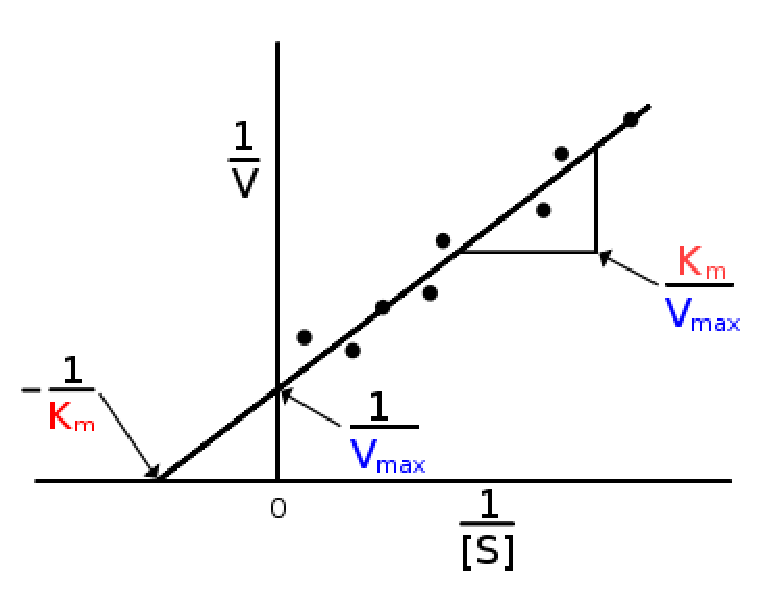
\includegraphics[height=5cm]{./images/Lineweaver-Burk_plot.eps}}
\caption{Lineweaver-Burk plot}
\label{fig:lineweaver-burk}
\end{figure}
$v$ achieve the value $v_\max$ only at very high [S].

{\bf NOTE}: Lineweaver-Burk even though provides interesting
interpretation, this method is error-prone. This is because of the
small error in the measurement of $v$ or $[S]$ can lead to
non-trivial error in $1/v_o$ and $1/[S]$. Thus, another method is more
preferable, e.g. Hanes-Woolf plot.


\subsection{* Hanes-Woolf plot}
\label{sec:Hanes-Woolf-plot}

{\bf Hanes-Woolf} plot plots
$[S]/v$ vs. $[S]$.
\begin{equation}
  \label{eq:324}
  \frac{[S]}{v} = \frac{1}{v_\max}[S] + \frac{K_m}{v_\max}
\end{equation}
Hanes-Woolf had been used to determined important kinetic parameters
$v_\max$, $K_m$, $v_\max/K_m$ rapidly. The drawback of Hanes-Woolf
is that both ordinate and abscissa are dependent variables of [S]; so
it is impossible to use statistical measurement (goodness of fit,
correlation coefficient R...) Nowadays, for a more accurate
computation, non-linear regressions are often being used.

$K_m$ for most enzymes is between $10^{-1}$ to $10^{-7}$ mM and
this values depends upon particular substrate as well as the
environment condition (pH, ionic strength, temperature). 

\subsection{Morrison kinetics: dynamic [S]}
\label{sec:morrison-kinetics}

When total enzyme concentration is significant compared to $K_m$, 
a significant fraction of substrate ([ES]) will be bound to the
enzyme. Thus, the substrate concentration [S] is no longer closed to
the total substrate $s_o$ (from the beginning), i.e. we need to use $[S] =
s_0-[ES]$.

Eq.\ref{eq:277} should be written as
\begin{equation}
  \label{eq:311}
  [ES]^2 - (e_0+s_0+K_m)[ES] + e_0s_0 = 0
\end{equation}
with $K_m=\frac{k_2+k_3}{k-1}$.

Finally, we have the rate of forming product 
\begin{equation} 
  \label{eq:312}
  v  = k_3 \ce{[ES]} =
  v_\max\frac{(e_0+s_0+K_m)-\sqrt{(e_0+s_0+K_m)^2-4e_0s_0}}{2e_0}
\end{equation}
with $v_\max = k_3 e_0$.

This quadratic velocity equation is aka {\bf tight-binding equation}
or Morrison equation~\citep{morrison1969kin}. As $K_m$ large, then the
quadratic equation approach the hyperbola curve of Michaelis-Menten
equation, as shown in Fig.~\ref{fig:Morrison_kin}.

\begin{figure}[hbt]
 \centerline{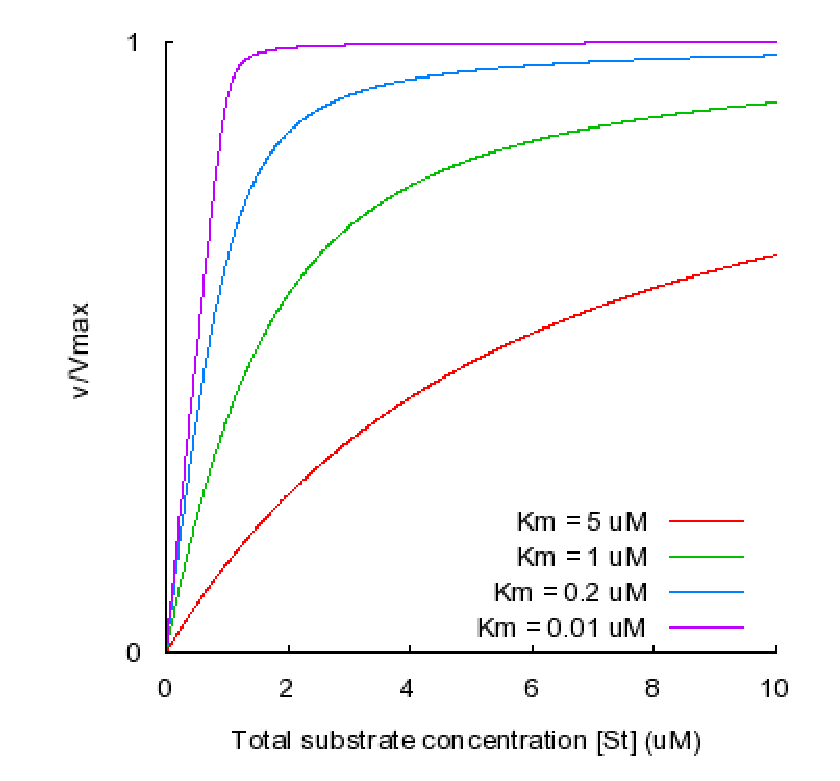
\includegraphics[height=5cm]{./images/Morrison_kin.eps}}
\caption{Morrison kinetics}
\label{fig:Morrison_kin}
\end{figure}

\subsection{Competitive one-site model}
\label{sec:competitive-one-site}

The competitive one-site model explains the situation when the binding site at
the enzyme can be bound by a molecule other the substrate, and this binding
inhibits the binding of the substrate.

This is similar to competitive two-site models
(Sect.~\ref{sec:competitive-two-site}), where the enzyme has one
catalytic binding site and one allosteric site and at a single
time, only one molecule can bind to the enzyme. So, the binding of the active
site prevents binding of the substrate and vice versa,
Fig.\ref{fig:enzyme_competitivemodel}.

\begin{figure}[hbt]
  \centerline{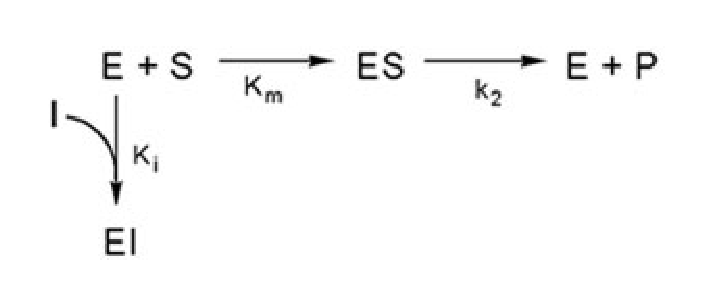
\includegraphics[height=3cm,
    angle=0]{./images/enzyme_competitivemodel.eps}}
\caption{An enzyme with one active site and one inhibitor: $K_i$ the
dissociation constant for EI complex}
\label{fig:enzyme_competitivemodel}
\end{figure}

The rate of production formation is now
\begin{equation}
v = k_3 \ce{[ES]} = v_\max \frac{\ce{[ES]}}{e_0} = v_\max
\frac{\ce{[S]}}{\ce{[S]} + K_m \left( 1 +
\frac{\ce{[I]}}{K_i} \right)}
\end{equation}

To see if the reaction following this scheme or not, we can use the following
plots: Michaelis-Menten, Lineweaver-Burk, and
Hanes-Woolf equations, with the equation modified to include a term that
describe the inhibition by I.
\begin{enumerate}
  \item Michaelies-Menten: $v = \frac{v_\max[\S]}{[S]+K_m\left(1 +
  \frac{[I]}{K_i} \right)}$
  \item Lineweaver-Burk: $\frac{1}{v} = \frac{1}{v_\max}+
  \frac{1}{v_\max}\frac{K_m}{[\S]}\left(1+\frac{[I]}{K_i}\right)$
  \item Hanes-Woolf: $\frac{[\S]}{v}=\frac{[\S]}{v_\max} +
  \frac{K_m}{v_\max}\left(1+\frac{[I]}{K_i}\right)$
\end{enumerate}

\subsection{Velocity of enzyme catalysis}
\label{sec:veloc-enzyme-catalys}

It's generally accepted that hydrolysis step is rate-limiting  in the
SR-ATPase reaction. In SERCA-pump, with a ``basic'' and a ``extra''
channels, the rate constants are the same, i.e. $k_h^b\approx
k_h^e=k_h$ (b=basic, e=extra). 

\begin{equation}
  \label{eq:1208}
  \ce{ATP + E1 <=> ATP\cdot E1}
\end{equation}
In the absence of $\Ca$, the velocity of enzyme catalysis with
saturating substrate concentration is
\begin{equation}
  \label{eq:1209}
  v_\max^{basic} = k_h^b[\ce{ATP\cdot E1}]\approx \frac{k_h[\ce{E0}]}{1+K_e}
\end{equation}
with $\ce{E0\approx[ATP\cdot E1]+[ATP\cdot E2]}$ is the total enzyme
concentration. 

In the presence of $\Ca$, the velocity of enzyme catalysis with
saturating substrate concentration is
\begin{equation}
  \label{eq:1210}
  v_\max^{total} = k_h^b[\ce{ATP\cdot E1}] + k_h^e[ADP\cdot P\sim E2]
  \approx [\ce{E0}]
\end{equation}
The extra maximal velocity is defined as
\begin{equation}
  \label{eq:1211}
  v_\max^{extra} = v_\max^{total}-v_\max^{basic} = k_h^e[ADP\cdot
  P\sim E2] \approx \frac{k_h[\ce{E0}]}{1+1/K_e}
\end{equation}

The plot log(V/T) vs. (1/T) are linear ``total'' ATPase, but not
nonlinear for ``basic'' and ``extra'' activities. 


% \section{Enzyme kinetics - other models}
% \label{sec:enzyme-kinet-other}
% 
% 
% To deal with the heterogeneous distribution of reactants, i.e. the
% fractal-like kinetics, there have been some limited mobility-derived
% kinetics have been successfully
% applied\footnote{\url{http://en.wikipedia.org/wiki/Michaelis-Menten_kinetics}}.
% For a single binding site model, 
% \begin{enumerate}
% \item when the substrate concentration $[\S]$ can change
%   (Sect.~\ref{sec:morrison-kinetics})
% \item the binding site at the enzyme can be bound by a molecule other
%   the substrate, that inhibit the binding of the substrate
%   (Sect.~\ref{sec:competitive-one-site}).
% \item as the enzyme is large, it can have more than one binding sites,
%   distinct from the active sites. The binding to these sites can
%   affect (enhance/degrade) the activity of the enzyme at the active
%   site. This is known as {\bf allosteric binding site} (or regulatory
%   sites). This is described in a separate section
%   (Sect.~\ref{sec:models-mult-bind}).
% \end{enumerate}
% 
% References:\url{http://assay.nih.gov/assay/index.php/Types_of_Inhibition}
% 
% \subsection{Lumped scheme of fast equilibrium}
% \label{sec:lumped-scheme-fast}
% 
% 


\section{Multiple-binding site approach}
\label{sec:models-mult-bind}

Both Michaelis-Menten kinetics, Briggs-Haldane kinetics and Morrison
kinetics use one-site model, in which each enzyme bind to a single
substrate only, and producing a product plus the enzyme
\begin{equation}
\ce{S + E -> P + E}
\end{equation}
In the simplest model, Michaelis-Menten, the enzyme activity is controlled by
the substrate concentration. In the Morrison model, the enzyme
activity is controlled by both the substrate and enzyme concentration.

\begin{framed}
\textcolor{red}{It's important to differentiate substrates vs. effectors}.
The site where substrate binding is called {\it catalytic site} (or active
site), while that for effector binding is called {\it regulatory site}.

  The broader term to refer to substrates and effectors is  {\bf ligand}, and
  both types of sites is called ligand-binding sites.

  If these substrate and effector  are identical, the interactions are
  termed {\bf homotrophic interactions}; otherwise, they are called
  {\bf heterotrophic interactions}. 
  
\end{framed}

As the enzyme is large, it can have more than one binding sites, i.e. more than
one substrates, and it can also produce more than one products.
In reality, many enzymes have more than one substrate (A, B) and more than one
product (P, Q). Substrates bind to catalytic sites; while Effectors bind to
regulatoric site(s). The binding to the regulatoric sites can affect
(enhance/degrade) the activity of the enzyme at the active  site.

Example: the enzyme alcohol dehydrogenase catalyzes the oxidation of
ethanol with NAD (a biological oxidizing agent) to form acetaldehyde and NADH.  

This makes the problem more complicated as there are different scenarios for the
binding to occur, and the products to be formed
\begin{enumerate}
  \item sequential yet random binding
  \item sequential yet ordered binding - Sect.\ref{sec:sequential-models}
  \item ping-pong mechanism - Sect.\ref{sec:ping-pong-mechanism}
\end{enumerate}

In an enzyme system, activating or inhibitory effects are measured in terms of
variations of the two classical kinetics constants ($K_m$ and $v_\max$), as a
function of the substrate concentration [S] and effector concentration [F].


\begin{framed}
  One-site models has the saturation curve as {\it hyperbolic},
  Fig.\ref{fig:hyperbolic_sigmoidal_relationship}.
  
  Multiple-site models has the saturation curve either (1) hyperbolic or (2)
  non-hyperbolic behavior (e.g. sigmoidal).   
\end{framed}

\subsection{Sequential binding
mechanism}
%\subsection{Sequential models}
\label{sec:sequential-models}

\textcolor{red}{In sequential models, the binding of all substrate is required
for product formation}. With multiple substrates (e.g. A and B) and multiple
binding sites, the binding at different sites on a single enzyme can be random
(A before B or B before A is the same) or in an ordered manner (A has to bind
before B). We will examine both cases, Fig.\ref{fig:binding-sequential}.

\begin{figure}[htb]
  \centerline{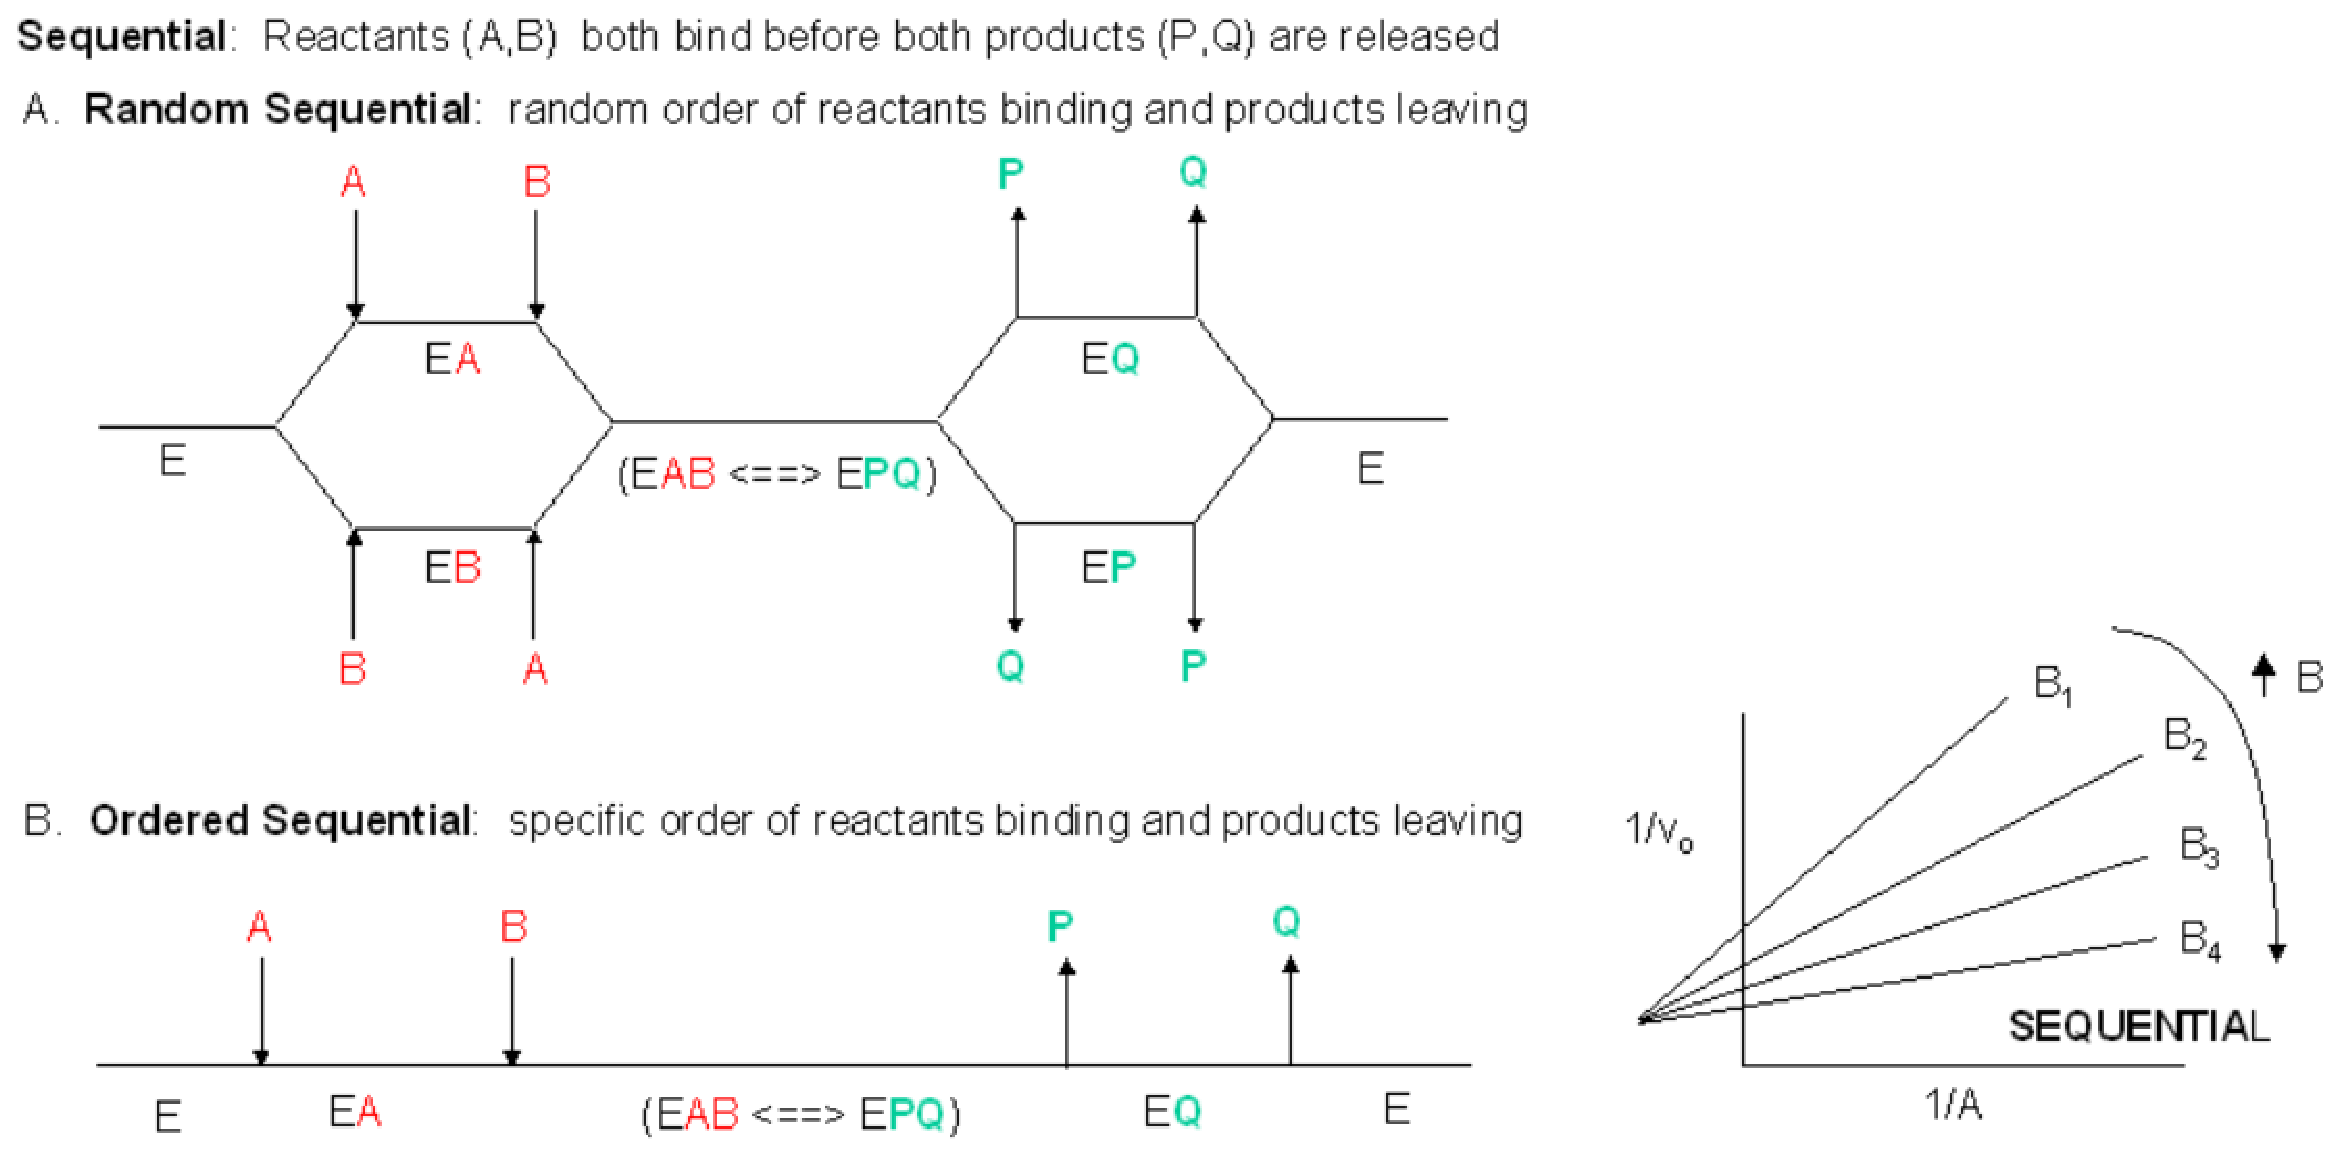
\includegraphics[height=4cm]{./images/binding_order2.eps}}
  \caption{(A) random sequential; (B) ordered
  sequential of binding with the signature
  Lineweaver-Burk plots $1/v$ vs. $1/\ce{[A]}$
  with different [B] concentrations intersected
  at a single point}\label{fig:binding-sequential}
\end{figure}

For both mechanisms, Lineweaver-Burk plots at varying A and different fixed
values of B give a series of intersecting lines,
Fig.\ref{fig:binding-sequential}.  Derivative curves can be solved to obtain
appropriate kinetic constants.

Early work in this regard was carried out by Adair and Pauling, operating under
the {\bf rapid equilibrium approximation}, i.e. 
all substrate binding and dissociation steps happen much more rapidly than
catalytically productive steps.

In 1954, King and Altman showed how to solve any kinetic system without
resorting to this approximation, but making it more complicated.
This is analogous to the difference between $K_M$ (or $K_D$) in the
Michaelis-Menten model and $K_M$ in the Briggs-Haldane model
(Sect.\ref{sec:quasi-steady-state}).


\subsection{* Sequential random model}
\label{sec:sequential-random-models}

\begin{figure}[htb]
  \centerline{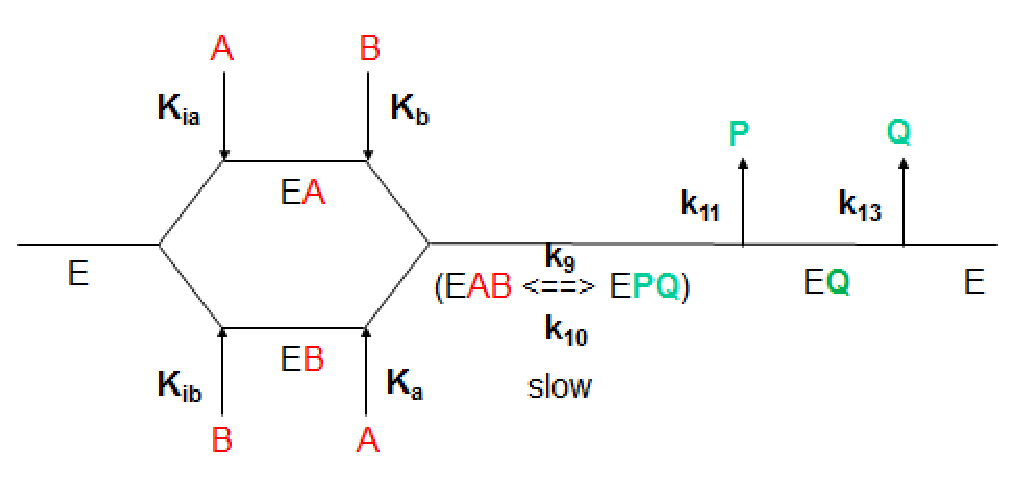
\includegraphics[height=5cm]{./images/sequential-random-binding.eps}}
  \caption{Sequential random binding}\label{fig:sequential-random-binding}
\end{figure}

Consider a random sequential bi-bi reaction for a "simple" case in which the
rapid equilibrium assumption defines the binding of substrates A and B,
Fig.\ref{fig:sequential-random-binding}. There are two effective dissociation
constant for the reactant A
\begin{itemize}
  \item $K_\text{ia}$: dissociation constant of A binding to E
  
  \item $K_\text{a}$: dissociation constant of A binding to EB
\end{itemize}

\begin{equation}
\begin{split}
\ce{E + A <->[K_{ia}] EA } \\
\ce{EA + B <->[K_b] EAB}
\end{split}
\end{equation}
or
\begin{equation}
\begin{split}
\ce{E + B <->[K_{ib}] EA } \\
\ce{EB + A <->[K_a] EAB}
\end{split}
\end{equation}

then
\begin{equation}
\begin{split}
\ce{EAB <=>[k_9][k_{10}] EPQ} \\
\ce{EPQ <->[k_{11}] P + EQ} \\
\ce{EQ <->[k_{13}] Q + E}
\end{split}
\end{equation}

The rate-limiting step is between \ce{EAB <=> EPQ}.

\begin{equation}
\begin{split}
\ce{K_{ia} = \frac{[E][A]}{[EA]}} \\
\ce{K_{ib} = \frac{[E][B]}{[EB]}} \\
\ce{K_{a} = \frac{[EB][A]}{[EAB]}} \\
\ce{K_{b}} = \frac{[EA][B]}{[EAB]} 
\end{split}
\end{equation}
from that we can find [E], [EA], [EB] as a function of [EAB].

NOTE: $e_0 = \ce{[E] + [EA] + [EB] + [EAB]}$, so
\begin{equation}
e_0 =  \left( \ce{\frac{K_{ia}K_b}{[A][B]} + \frac{K_b}{[B]} + \frac{K_a}{[A]}
+1} \right) \ce{[EAB]}
\end{equation}

NOTE: Assuming rapid equilibrium of the two paths, i.e. all substrate binding
and dissociation steps happen much more rapidly than catalytically productive
step, then $\ce{K_{ia}K_b = K_{ib}K_a}$.


References:
\begin{itemize}
  \item
  \url{http://employees.csbsju.edu/hjakubowski/classes/ch331/transkinetics/olcomplicatedenzyme.html}
\end{itemize}

\subsection{* Sequential ordered model}
\label{sec:sequential-ordered-models}
%(Random-Sequential vs. Ordered-Sequential) 

For random reactions the order in which the substrates bind does not matter. 
Although sequential ordered models are less general than sequential random
models, they have fewer free parameters and so are easier to use when fitting
experimental data. This means that, \textcolor{red}{in cases where they are
applicable, sequential ordered models
  are often a better choice than sequential random models when it comes to
  analyzing experimental data}~\citep{monod1965nat}.

An abbreviated notation  scheme developed by W.W. Cleland is shown below for the
sequential random and sequential ordered mechanisms.  

\subsection{* Sequential: single subtrate but multi-binding sites and one
product}

Fig.\ref{fig:single-substrate-multi-bindingsite_single-product} shows a model in
which the enzyme has two binding sites, that can accept a single type of
substrate
\begin{itemize}
  \item the first binding of S, forming complex ES that can produce product P,
  with rate $k_\text{cat}$
  
  \item the second binding of S, forming doubly-occupied complex ESS that can
  produce product P, but tentatively with a faster rate $k_\text{cat2}$.
\end{itemize}

 \begin{figure}[htb]
  \centerline{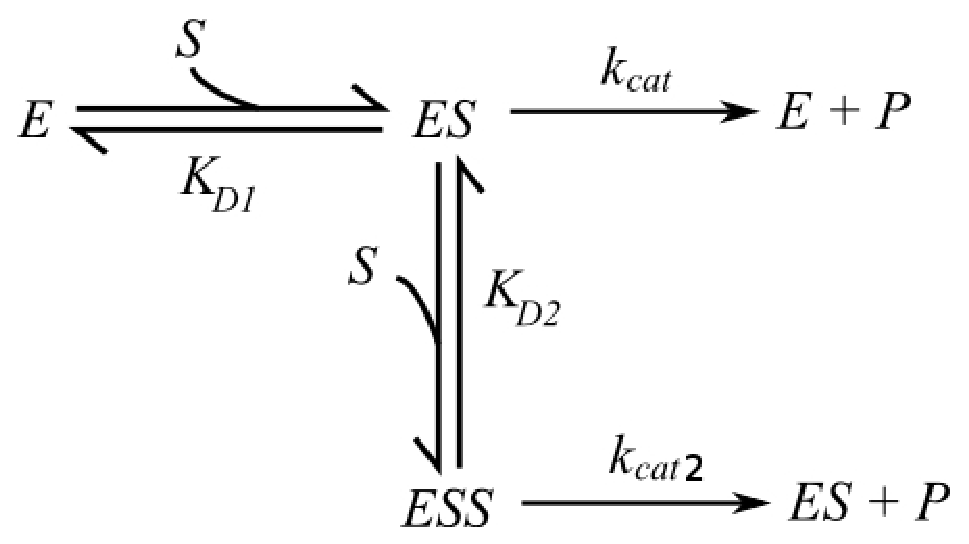
\includegraphics[height=4cm]{./images/single-substrate-multi-bindingsite_single-product.eps}}
  \caption{Single
  subtrate, with
  multiple binding
  sites, e.g. two,
  and one product}\label{fig:single-substrate-multi-bindingsite_single-product}
\end{figure}

Under the assumption of fast equilibrium of substrate
association/disassociation
\begin{equation}
\begin{split}
\ce{K_{d1} = \frac{[E][S]}{[ES]} } \\
\ce{K_{d2} = \frac{[ES][S]}{[ESS]} }
\end{split}
\end{equation}

From that we can calculate [ES],
[ESS].
\begin{equation}
\begin{split}
\ce{[ES] = \frac{[E][S]}{K_{d1}}  } \\
\ce{[ESS] = \frac{[ES][S]}{K_{d2}}} = \frac{[E][S]^2}{K_{d1}{K_{d2}}} 
\end{split}
\end{equation}
NOTE: $e_0 = \ce{[E] + [ES] + [ESS]}$, so we need to find [E] as a function of
$e_0$, and then replace into the previous equations to find [ES] and [ESS] as a
function of $e_0$
\begin{equation}
e_0 = \ce{[E]} \left( 1 + \ce{\frac{[S]}{K_{d1}} + \frac{[S]^2}{K_{d1}K_{d2}}}
\right)
\end{equation}
or
\begin{equation}
\begin{split}
\ce{[ES] =  ...   } \\
\ce{[ESS] =  ...   }
\end{split}
\end{equation}


Finally, the reaction velocity $v$:
\begin{equation}
v = \ce{ k_{cat} [ES] + k_{cat,2}[ESS] } =
\ce{ \frac{k_{cat} \frac{[S] e_0}{K_{d1}}  + k_{cat,2}
\frac{[S]^2 e_0}{K_{d1}K_{d2}} }{1 + \frac{[S]}{K_{d1}} +
\frac{[S]^2}{K_{d1} K_{d2}} } }
\end{equation}

NOTE:
\begin{equation}
v_{\max,1} = k_\text{cat} \ce{e_o} \;\;\;
v_{\max,2} = k_\text{cat2} \ce{e_o} 
\end{equation}

then the equivalent form
\begin{equation}
v = \ce{ v_{\max,1}[ES]/e_0 + v_{\max,2}[ESS]/e_0 } =
\frac{v_{\max,1} \frac{[S]}{K_{d1}}  + v_{\max,2} \frac{[S]^2}{K_{d1}K_{d2}} }
{1 + \frac{[S]}{K_{d1}} +\frac{[S]^2}{K_{d1} K_{d2}} }  
\end{equation}


\url{http://depts.washington.edu/wmatkins/kinetics/sequential.html}

\subsection{Non-sequential binding}

Non-Sequential mechanism does not require both substrates to bind before
releasing the first product. 
Typically, the binding of the second substrate could result
in a change of the shape of the first substrate saturation curve that makes
production more effective or less effective.

\begin{enumerate}
  \item Ping-pong mechanism - Sect.\ref{sec:ping-pong-mechanism}
\end{enumerate}

\subsection{* Ping-pong binding mechanism (double-displacement mechanism)}
\label{sec:ping-pong-mechanism}

Ping-pong mechanism is a type of non-sequential binding. 
It is called this because the enzyme bounces back and forth from an intermediate
state to its standard state. Here, we have two substrates A and B; binding 
(at potentialy two different sites) on enzyme E, to form two products P and Q.

The substrate A binds first to the enzyme and produce product P.
{\it Typically, this is the scenario when the product P is a fragment of the
original substrate A}; and the rest of the substrate is covalently attached to
the enzyme E , which is designated as E'.

\begin{equation}
\ce{A + E -> EA <=> P.E^' -> P + E^'}
\end{equation}

The product P is a fragment of A; and the other fragment of A still
attaches to the enzyme, giving E'.

Now the second reactant, B, binds and reacts with E' (e.g. B forms a covalent
bond to the fragment of A still attached to the enzyme), from that the
product Q is created.
\begin{equation}
\ce{B + E^' -> E^'B <=> EQ -> Q + E}
\end{equation}

\begin{figure}[htb]
  \centerline{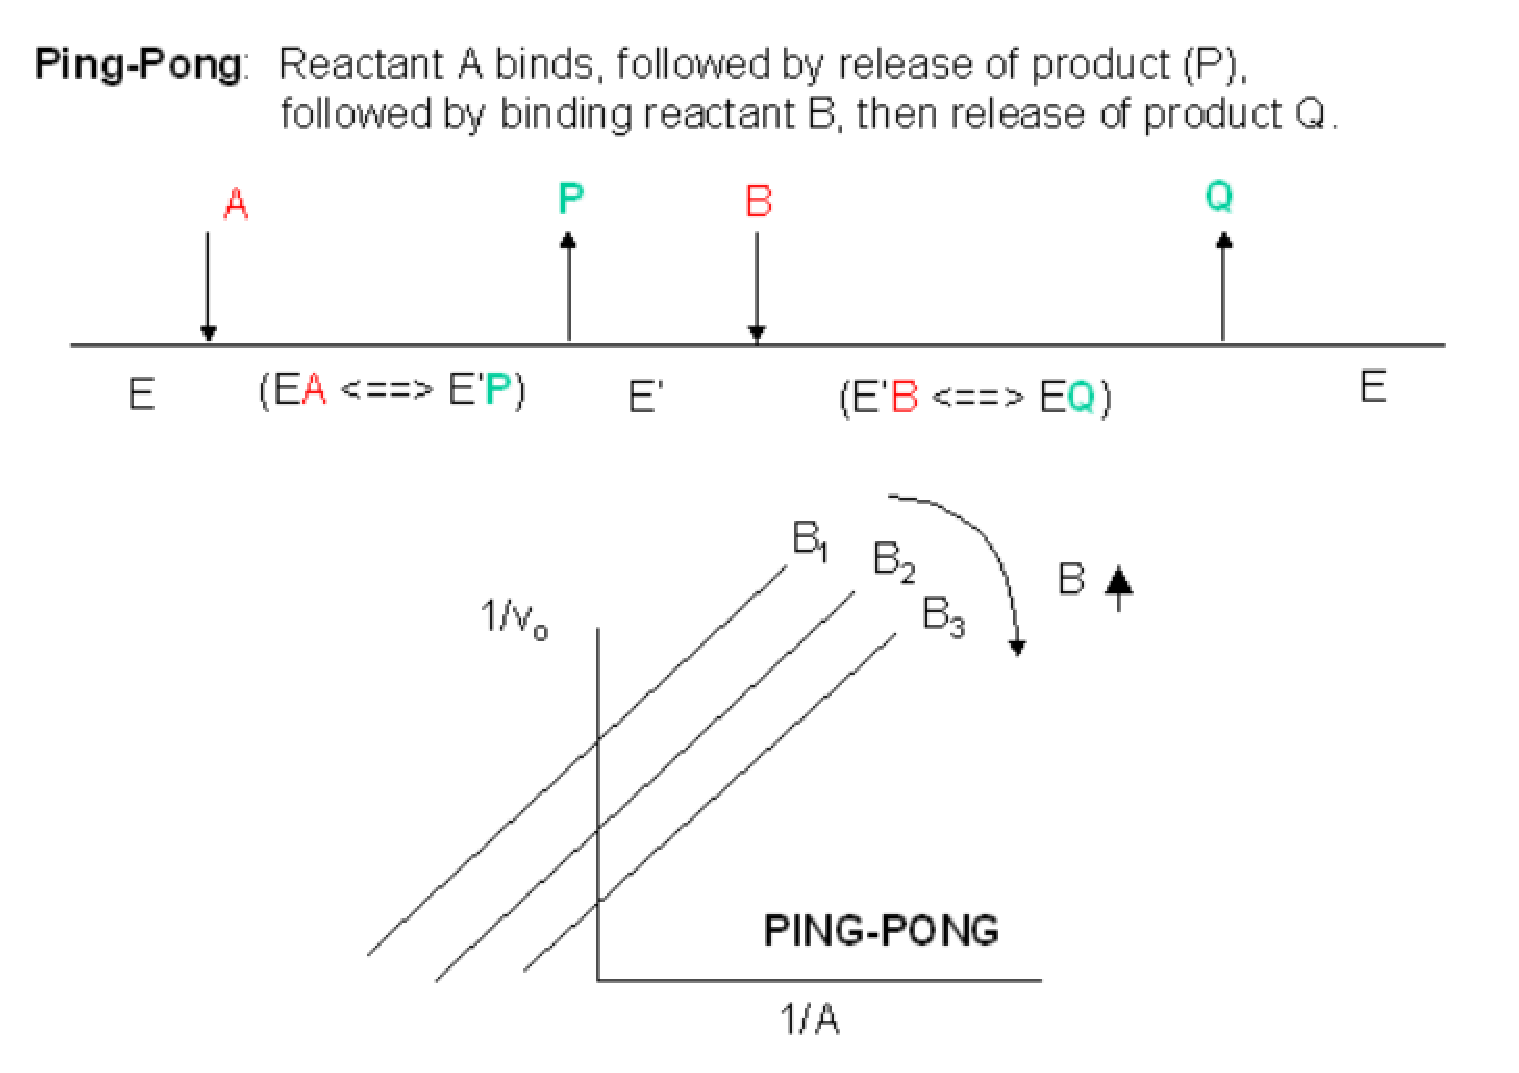
\includegraphics[height=4cm]{./images/pingpong-mechanism.eps}}
  \caption{Ping-pong mechanism with the signature
  parallel lines in Lineweaver-Burk plot of $1/v$
  vs. $1/\ce{[A]}$ curves at different [B]
  concentrations}\label{fig:pingpong-mechanism}
\end{figure}

This represents a {\bf ping-pong mechanism} or {\bf double-displacement
mechanism}, Fig.\ref{fig:pingpong-mechanism}. The enzyme exists in an
intermediate form E' which is temporary and at the end of the reaction the
enzyme MUST be found in its original form.

\begin{equation}
\begin{split}
\ce{A + E -> EA <=> P.E^' -> P + E^' } \\
\ce{B + E^' -> E^'B <=> EQ -> Q + E}
\end{split}
\end{equation}

\textcolor{red}{How to identify}: 
For this mechanism, Lineweaver-Burk plots
(Sect.\ref{sec:Lineweaver-Burk-plot}) at varying A and different fixed values of
B give a series of parallel lines, i.e. the plot of $1/v$ vs. $1/\ce{[A]}$ as
[B] changes.

\url{http://chemwiki.ucdavis.edu/Biological_Chemistry/Catalysts/Enzymatic_Kinetics/Ping-pong_mechanisms}

\subsection{Meaning of $K_m$, velocity $v$ in multi-substrate/multi-product
mechanism?}


\subsection{Meaning of $K_m$, velocity $v$ in allosteric mechanism?}

\subsection{K system vs. V system}

In both K and V systems, an effector can act as an activator (positive effector)
or an inhibitor (negative effector).

\subsection{* K system: competitive-binding (change $K_m$)}


If the binding of a ligand (effector, substrate) involves the change
in Michaelis-Menten constant $K_m$ but no change in maximal velocity,
the effect of the ligand is ``competitive'' and the system is called
{\bf K system}, as shown in Fig. \ref{fig:K_system}. 

\begin{figure}[hbt]
 \centerline{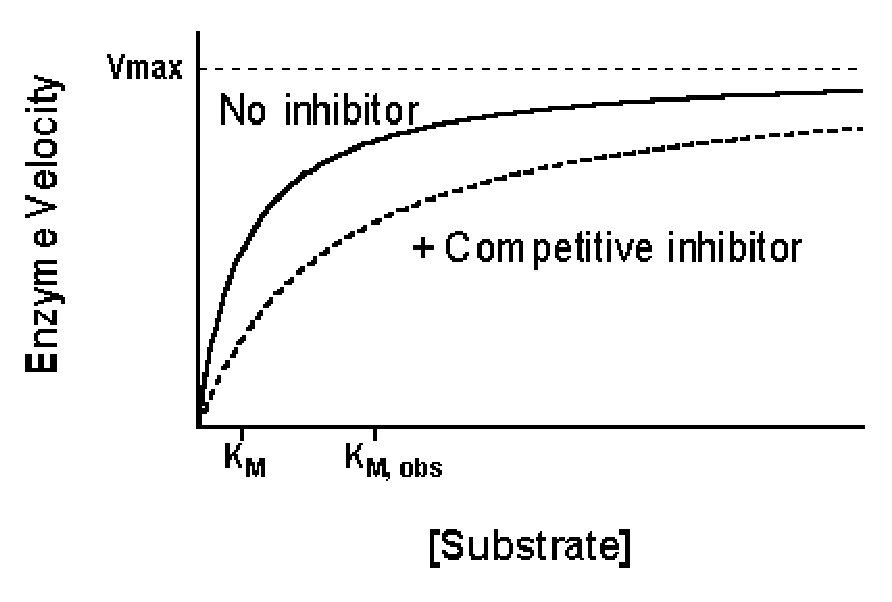
\includegraphics[height=5cm]{./images/K_system.eps}}
\caption{K system}
\label{fig:K_system}
\end{figure}

\subsection{* V system: uncompetitive binding (change $v_\max$)}


Similarly, if the
binding of a ligand involves the change in maximal velocity only, the
effect of the ligand is ``uncompetitive'' and the system is referred
to as {\bf V system} ~\citep{monod1965nat}. 

\begin{figure}[hbt]
 \centerline{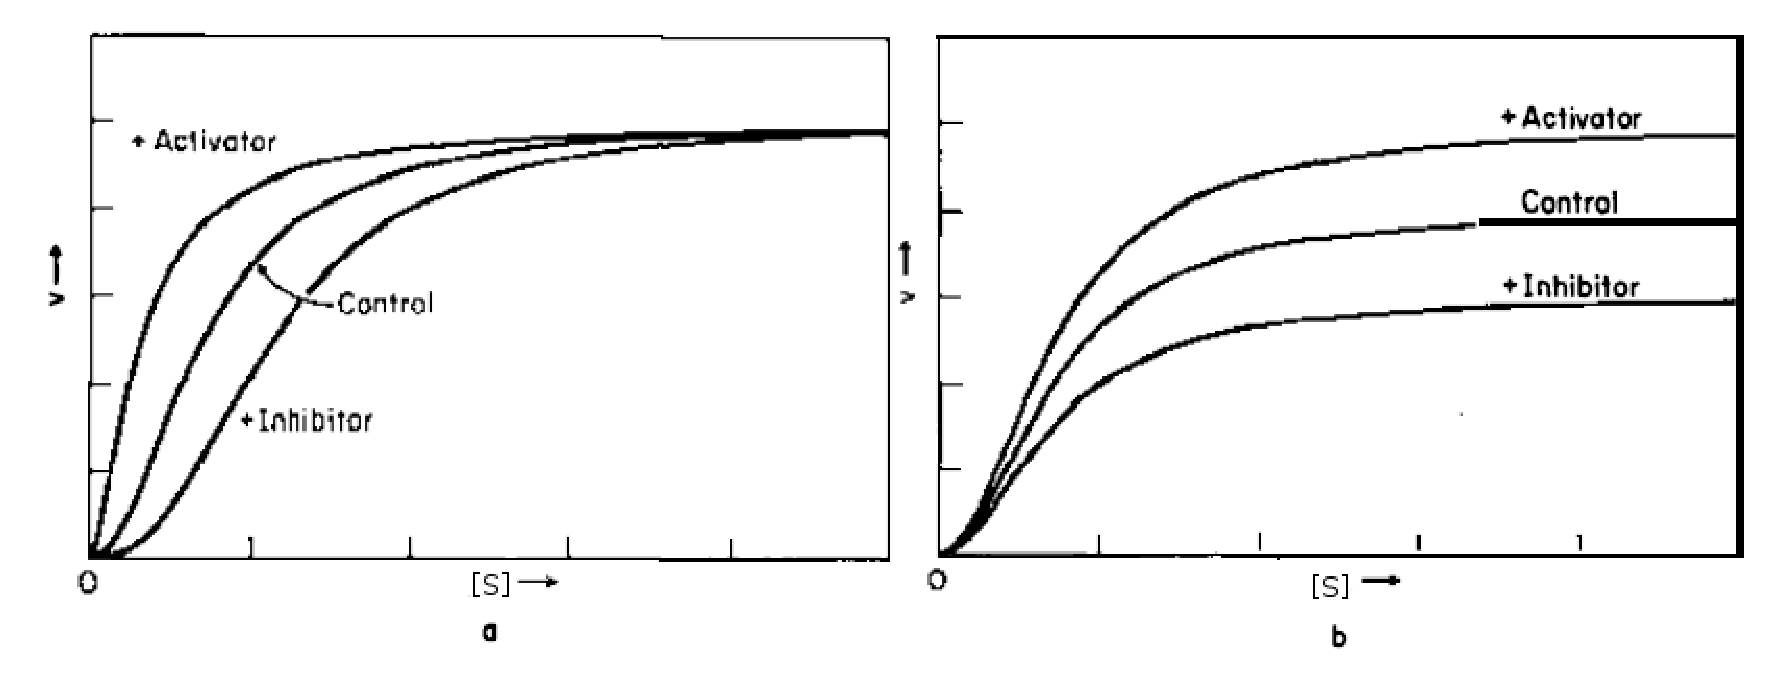
\includegraphics[height=5cm]{./images/Allosteric_enzyme_K_V.eps}}
 \caption{Behavior of allosteric systems: (A) K-system; (B)
   V-system. $v$ is the initial velocity of the enzymatic reaction and
   [$L$] is the ligand concentration}
\label{fig:enzyme_K_V}
\end{figure}

This is known as {\bf allosteric binding site} (or regulatory
sites).


Allosteric interactions (between enzyme and effectors) stabilize
conformational state of the enzyme that either increase/decrease the
affinity for substrate (K-system) or catalytic potential (V-system) or
both, as shown in Fig.~\ref{fig:enzyme_K_V}. Allosteric interactions
play an important role in the regulation of enzyme
activity~\citep{hammes1973kae}.

\subsection{Allosteric (cooperativity) binding: K }


\begin{figure}[htb]
  \centerline{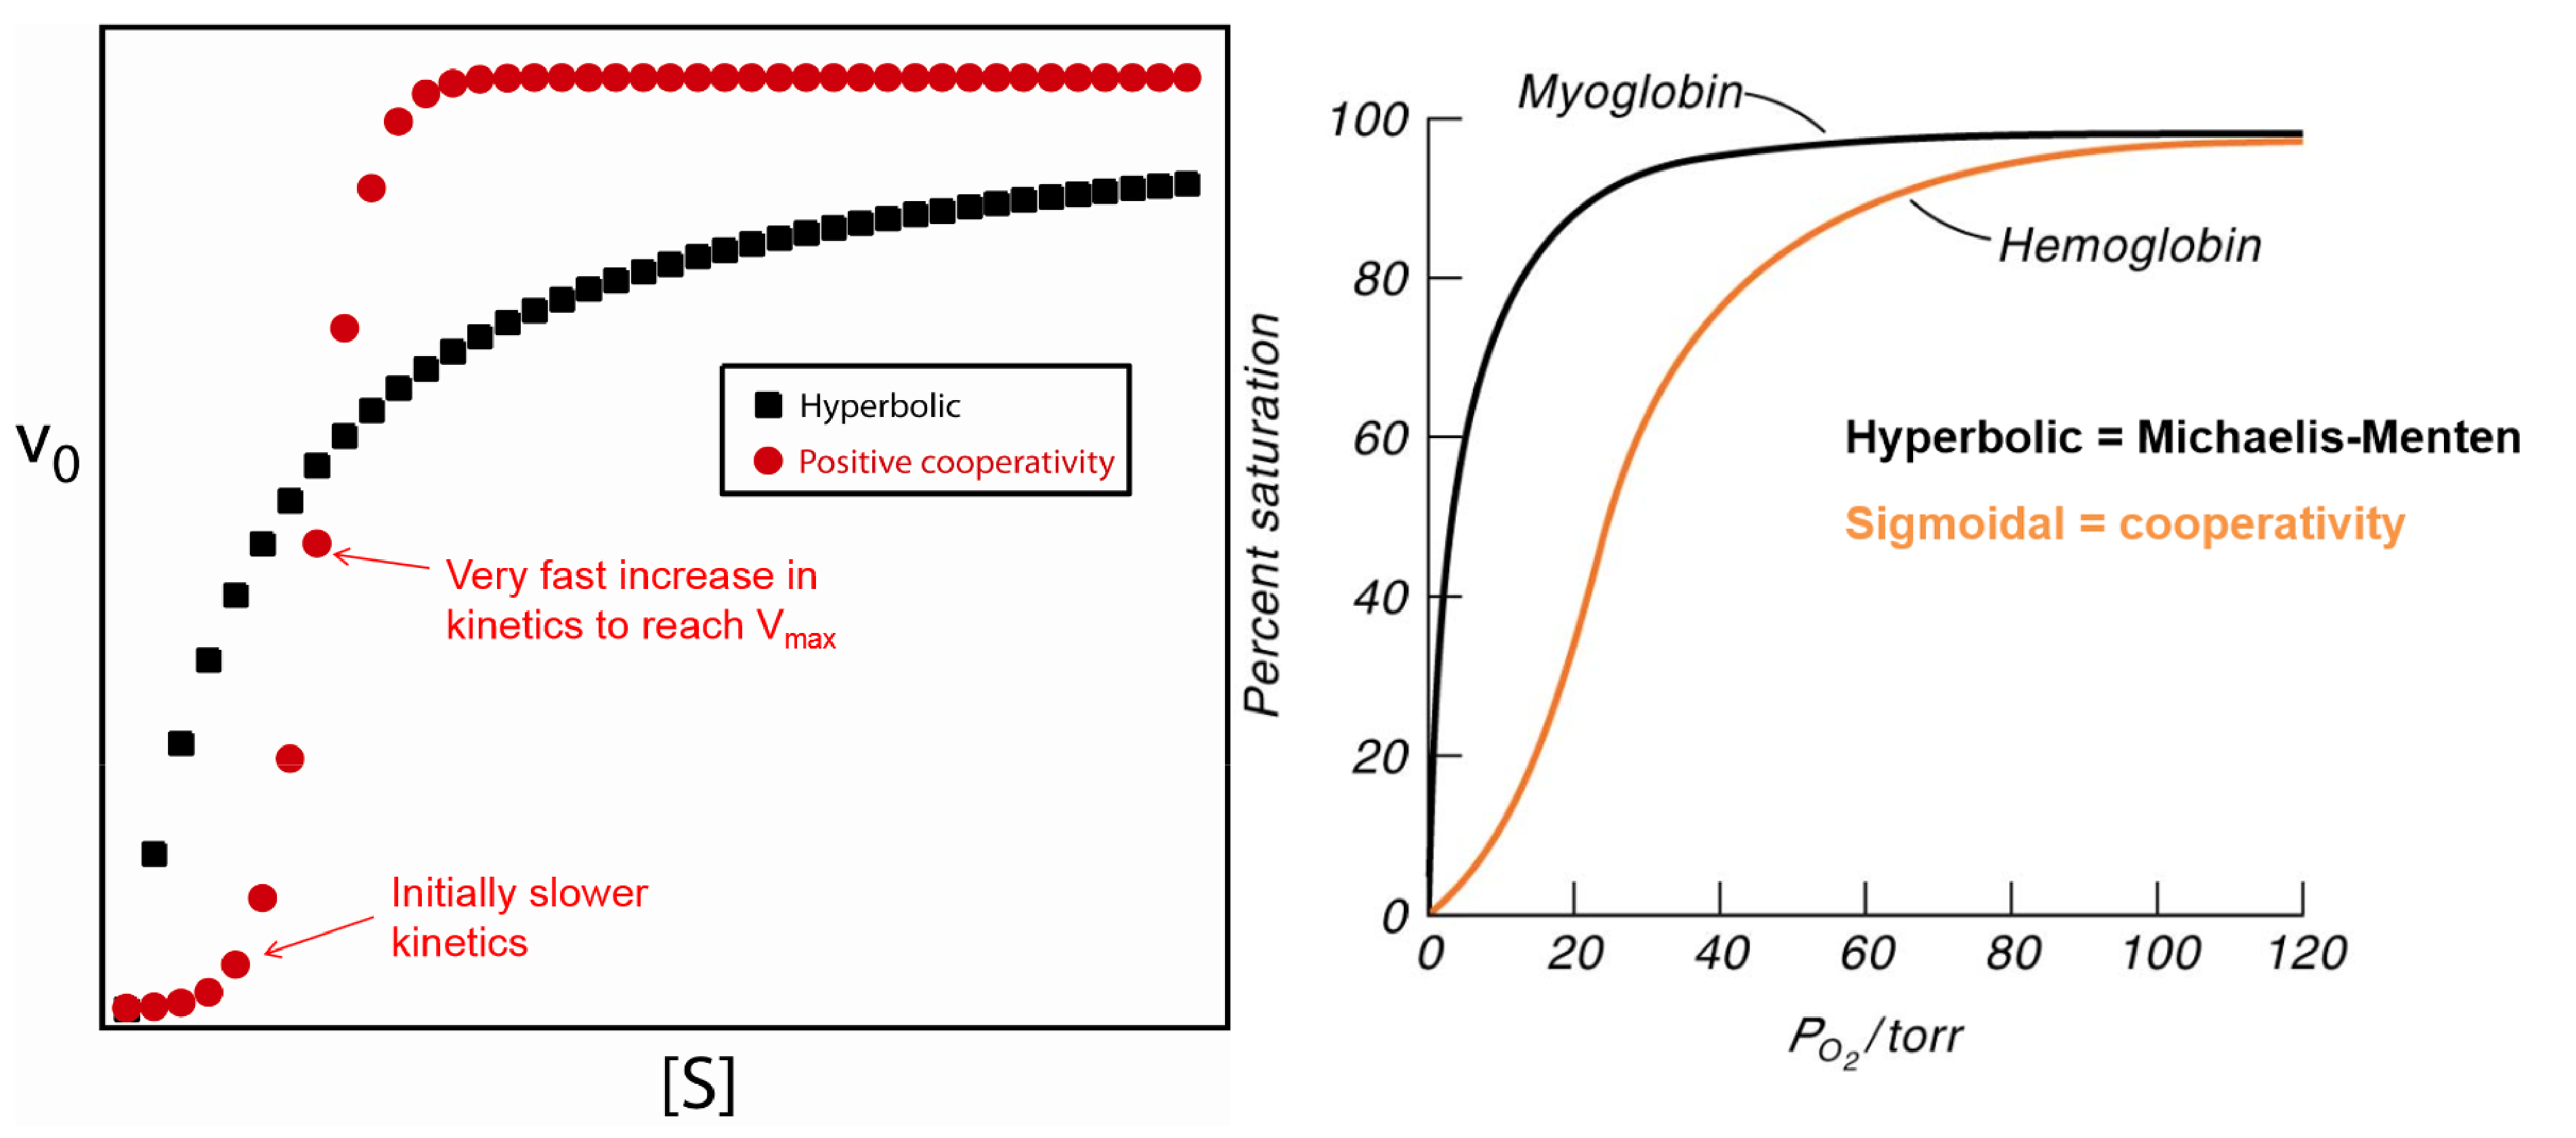
\includegraphics[height=5cm]{./images/hyperbolic_sigmoidal_relationship.eps}}
  \caption{Hyperbolic
  (Michaelis-Menten)
  vs. Sigmoidal
  (Cooperativity)}\label{fig:hyperbolic_sigmoidal_relationship}
\end{figure}

  In reality, many of regulatory enzyme exhibit {\it non-hyperbolic}
kinetic and/or binding isotherms. Such behavior can be explained as
the activity is enhanced or degraded by the binding of some other
molecules. This can be multiple substrate or effector binding sites on
the enzyme~\citep{hammes1973kae}. The effector can be either
activators or inhibitors that correspondingly enhance or inhibit the
activity of the associated enzyme.
  

  In multiple-binding models, the binding of the first ligand can
  enhance/facilitate the binding to the second ligand (``positive
  cooperativity'' - the curve has {\it sigmoidal shape}); or the binding
  can inhibit the binding to the second (``negative cocoperativity'' - the
  curve has inverse sigmoidal shape),
  Fig.\ref{fig:hyperbolic_sigmoidal_relationship}.

\subsection[Non-competitive two-site model]{Non-competitive two-site model: one
substrate + one inhibitor}
\label{sec:non-competitive-two}

\begin{figure}[hbt]
  \centerline{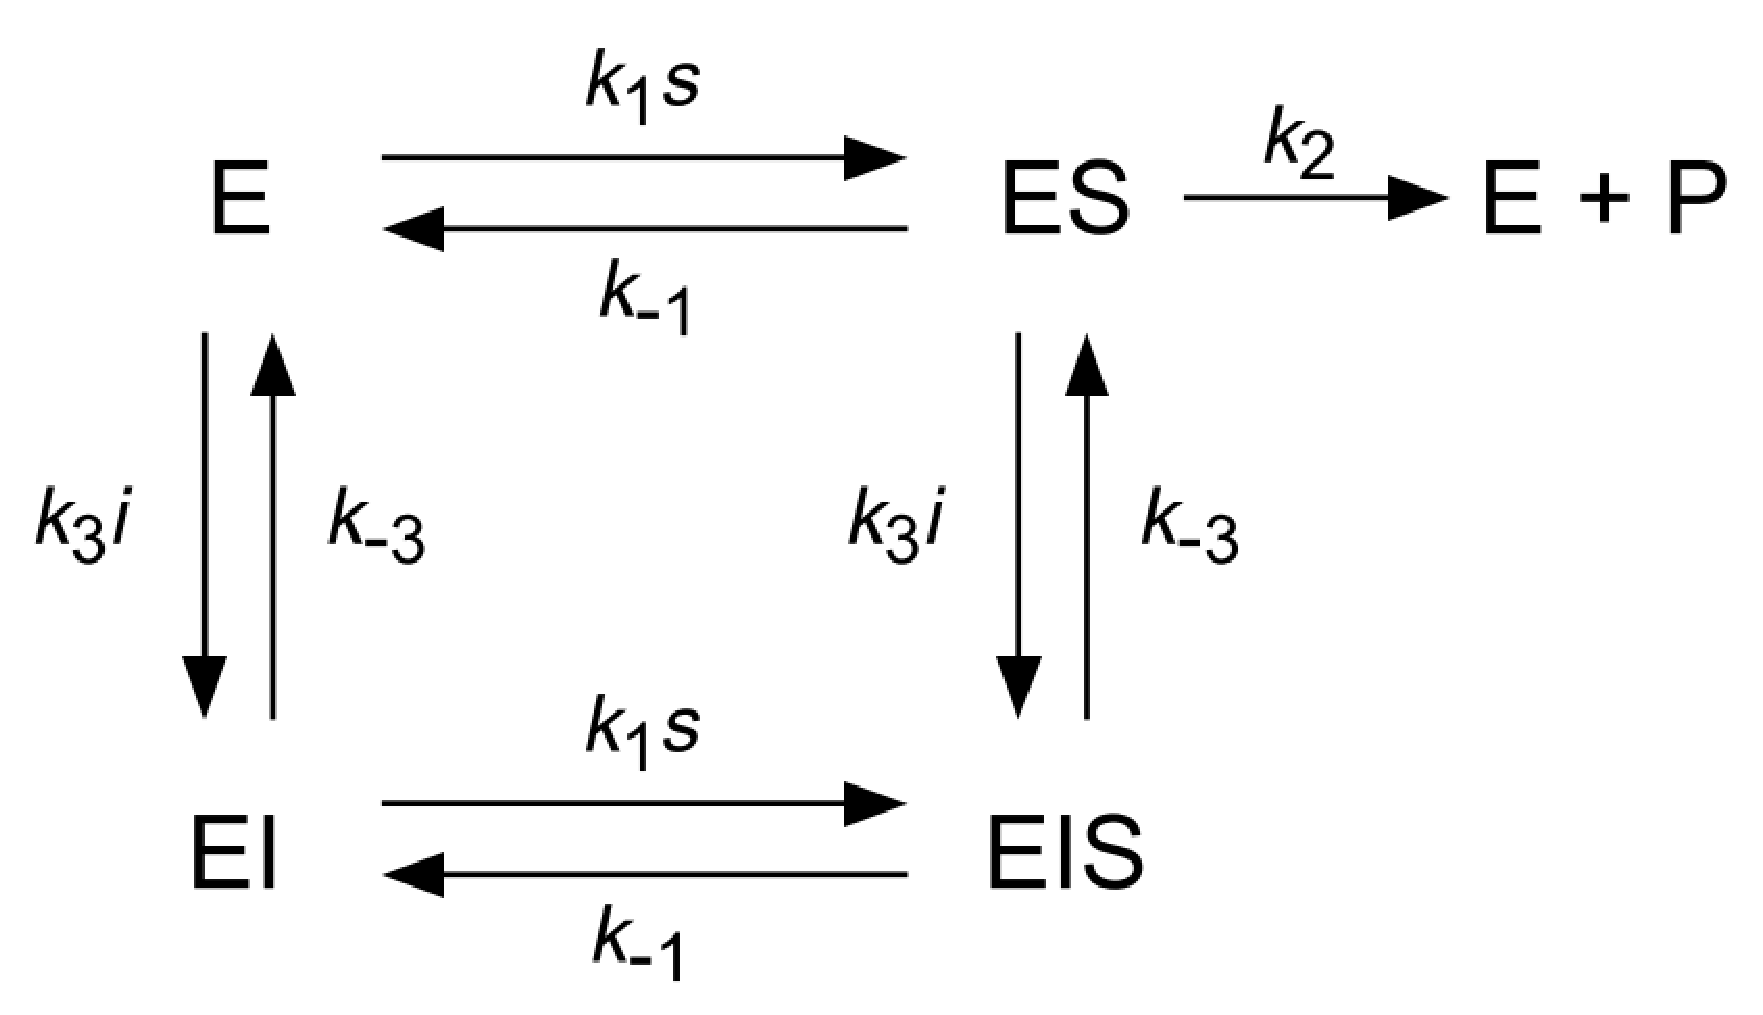
\includegraphics[height=5cm,
    angle=0]{./images/1bind_1inhibit.eps}}
  \caption{An enzyme with 1 catalytic binding site and 1 allosteric
    one}
\label{fig:1bind_1inhibit}
\end{figure}

In this situation, the enzyme has two binding sites, one for substrate
and one for inhibitor. Thus, both enzyme (E) and the complex (ES) can
also interact with the inhibitor ($I_c$),
Fig.~\ref{fig:1bind_1inhibit}. 

By using Lineweaver-Burk plot, it is observed that competitive
inhibitors decrease $v_\max$ but have no effect on $K_m$,
Fig.~\ref{fig:enzyme_K_V}(b). The new maximum velocity $v'_\max$ has
the relation with the old $v_\max$ as follows
\begin{equation}
  \label{eq:326}
  v'_\max = \frac{1}{1+\frac{[I_c]}{K_i}} v_\max
\end{equation}
with $K_i=\frac{k^-_3}{k^+_3}$.  Then, the new initial velocity
formula is
\begin{equation}
  \label{eq:327}
  v = \frac{1}{1+\frac{[I_c]}{K_i}} v_\max \frac{[S]}{K_m+[S]}
\end{equation}
with $v_\max = k_2[\text{E}]_o$.

As shown in Fig.~\ref{fig:enzyme_K_V}(b), the curve $v$ vs. [S]
looks very different from a competitive inhibitor since increasing [S]
has no impact on the increase in the initial velocity. A negative
cooperativity can also decrease maximum velocity
(Sect.~\ref{sec:negat-coop}).

\subsection[Competitive two-site model]{Competitive two-site model: one substrate + one inhibitor}
\label{sec:competitive-two-site}

An enzyme mechanism model for the enzyme with one site for substrate,
but now with an inhibitor that is competitive to bind to the same
site on the enzyme. The binding of the inhibitor prevent the binding
of the substrate to the enzyme. This is the model for the competitive
inhibitor ($I_C$) interacting with the enzyme (E). This is aka the K
system. 
\begin{equation}
  \label{eq:323}
  \begin{split}
    &\ce{E  + S <=>[k_1][k_2] ES ->[k_3] E + P} \\
    &+ \\
    &I_C \\
    &\upharpoonleft\downharpoonright K_i \\
    & EI_C
  \end{split}
\end{equation}
with $K_i$ is the inhibitor binding constant.
Due to the binding of inhibitor, it slows down the process, thus the
$v$ vs. $[S]$ curve change with the presence of competitive
inhibitor. 

With the presence of inhibitors, the
\textcolor{red}{new Michaelis-Menten constant is $K'_M$ which has a
  relation to the old $K_m$} as follows
\begin{equation}
  \label{eq:325}
  K'_M = K_m \left( 1 + \frac{[I_c]}{K_i} \right)
\end{equation}
Then, the new initial velocity formula
is~\citep{dixon1953eic,kakkar1999cei}
\begin{equation}
  \label{eq:328}
  v =  v_\max \frac{[S]}{ K_m \left( 1 + \frac{[I_c]}{K_i} \right)+[S]}
\end{equation}
with $K_m=\frac{k_1+k_2}{k_3}$.



\subsection{Multiple catalytic binding sites - independent}
\label{sec:mult-catalyt-bind}

Consider an enzyme with $n$ catalytic binding sites for ligand
L. Then, we will have $n$ corresponding association constant $K_i$.
\begin{equation}
  \label{eq:313}
  \begin{split}
    E + L &\ce{<=>} EL; \; K_1 = \frac{[EL]}{[E][L]} \\
    EL + L &\ce{<=>} EL_2; \; K_2 = \frac{[EL_2]}{[EL][L]} \\
    \vdots \\
    EL_{n-1} + L &\ce{<=>} EL_n; \; K_n = \frac{[EL_{n}]}{[EL_{n-1}][L]} 
  \end{split}
\end{equation}
The average number $r$ of ligand molecules bound to the enzyme is
defined as
\begin{equation}
  \label{eq:314}
  \begin{split}
      r &= \frac{\text{moles of L bound}}{\text{moles of enzyme}} =
  \frac{\sum^n_{i=1} i[PL_i]}{\sum_{i=0}^n [PL_i]} \\
  &= \frac{K_1[L]+2K_1K_2[L]^2 + \dots +
    nK_1...K_n[L]^n}{1+K_1[L]+K_1K_2[L]^2+\dots + K_1K_2...K_n[L]^n}
  \end{split}
\end{equation}
This is aka {\bf Adair equation}~\citep{adair1925odc}. This is general,
however, quite complex when $n$ is large.
\textcolor{red}{A common assumption is given to simplified it: all
  sites are independent and identical}.
Thus, the intrinsic association constant are the same $K$ which
relates to the association constant defined above as
\begin{equation}
  \label{eq:315}
  K_i = \frac{n-i+1}{i} K; \; i\ge 1
\end{equation}
Finally, we have
\begin{equation}
  \label{eq:316}
  r = \frac{nK[L]}{1+K[L]}
\end{equation}

The identical sites are classified into a single class. For a single
type of ligand L, most enzymes indeed, have more than two classes of
binding sites. Thus, if the enzyme has $n_1$ equivalent sites of class
1 with an intrinsic association constant $K_1$, $n_2$ equivalent sites
of class 2 with an intrinsic association constant $K_2$..., and the
binding to each class of sites occurs independently, then with $m$
classes of binding sites, we have
\begin{equation}
  \label{eq:317}
  r = \sum_{i=1}^m r_i = \sum_{i=1}^m \frac{n_iK_i[L]}{1+K_i[L]}  
\end{equation}
This adequately describes the data, but not provide any explanation
for the changing association constants. To establish a nature of the
cooperativity between binding sites, different methods of plotting
binding data have been utilized. The curves from 1-4 are shown in
Fig.~\ref{fig:enz_kin}, the curve in 5 is shown in
Fig.~\ref{fig:enz_kin_2}.
\begin{enumerate}

\item $r$ vs. [L]: 
  \begin{itemize}
  \item If enzyme contains only identical sites (single class of
    sites)
    \begin{itemize}
    \item For non-interacting cooperativity, a hyperbolic curve is
      obtained.
    \item For positive cooperativity, the curve is sigmoidal
    \item For negative cooperativity, the final value of $r$ approach
      more slowly than in a hyperbolic curve.
    \end{itemize}
  \item If enzyme contains more than two classes of binding sites,
    both positive and negative cooperativities are possible and the
    plots may display undulation or bumps~\citep{teipel1969ipr}
  \end{itemize}

\item $r$ vs. $\log([L])$: By using log, this plot can cover a wide
  range of concentration [L], and the steepness of the curve can give
  a convenient measure of the cooperativity.
  \begin{itemize}
  \item all binding isotherms (curves) appears in sigmoidal
  \item equal steepness for equal
    cooperativity~\citep{koshland1966ceb}.
  \item the steepness is in the order of {\it positive cooperativity}
    $>$ {\it no cooperativity} $>$ {\it negative cooperativity}
  \end{itemize}

\item $1/r$ vs. $1/[L]$:
  \begin{itemize}
  \item linear for non-interacting identical sites (single class); and
    the slope is $\frac{1}{nK}$, the intercept is $1/n$.
  \item concave upward for positive cooperativity 
  \item concave downward for negative cooperativity. However, this can
    also be obtained from polymorphic forms, electrostatic
    repulsion.... So, the concave downward cannot be used as a proof
    of negative cooperativity.
  \end{itemize}

\item $\frac{r}{[L]}$ vs. $r$: the equivalent form of
  eq.~\eqref{eq:316} is
  \begin{equation}
    \label{eq:318}
    \frac{r}{[L]} = Kn - Kr
  \end{equation}
This plot is called {\bf Scatchard plot}, a convenient for determining
both $n$ and $K$.
\begin{itemize}
\item linear for non-interacting identical sites
\item concave downward for positive cooperativity
\item concave upward for negative cooperativity
\end{itemize}

\item $\log\frac{r}{n-r}$ vs. $\log([L])$: As mentioned in the
  previous section, the sigmoidal curve can also be fitted by the Hill
  equation
  \begin{equation}
    \label{eq:319}
    r = \frac{n[L]^h}{K + [L]^h}
  \end{equation}
with $h$ is the Hill coefficient; the equivalent form is
\begin{equation}
  \label{eq:320}
  \log\frac{r}{n-r} =h\log[L] - \log K
\end{equation}
\begin{itemize}
\item Hill coefficient $h> 1$: positive cooperativity
\item Hill coefficient $h= 1$: no-interacting cooperativity
\item Hill coefficient $h< 1$: negative cooperativity
\end{itemize}
\end{enumerate}

\begin{figure}[hbt]
 \centerline{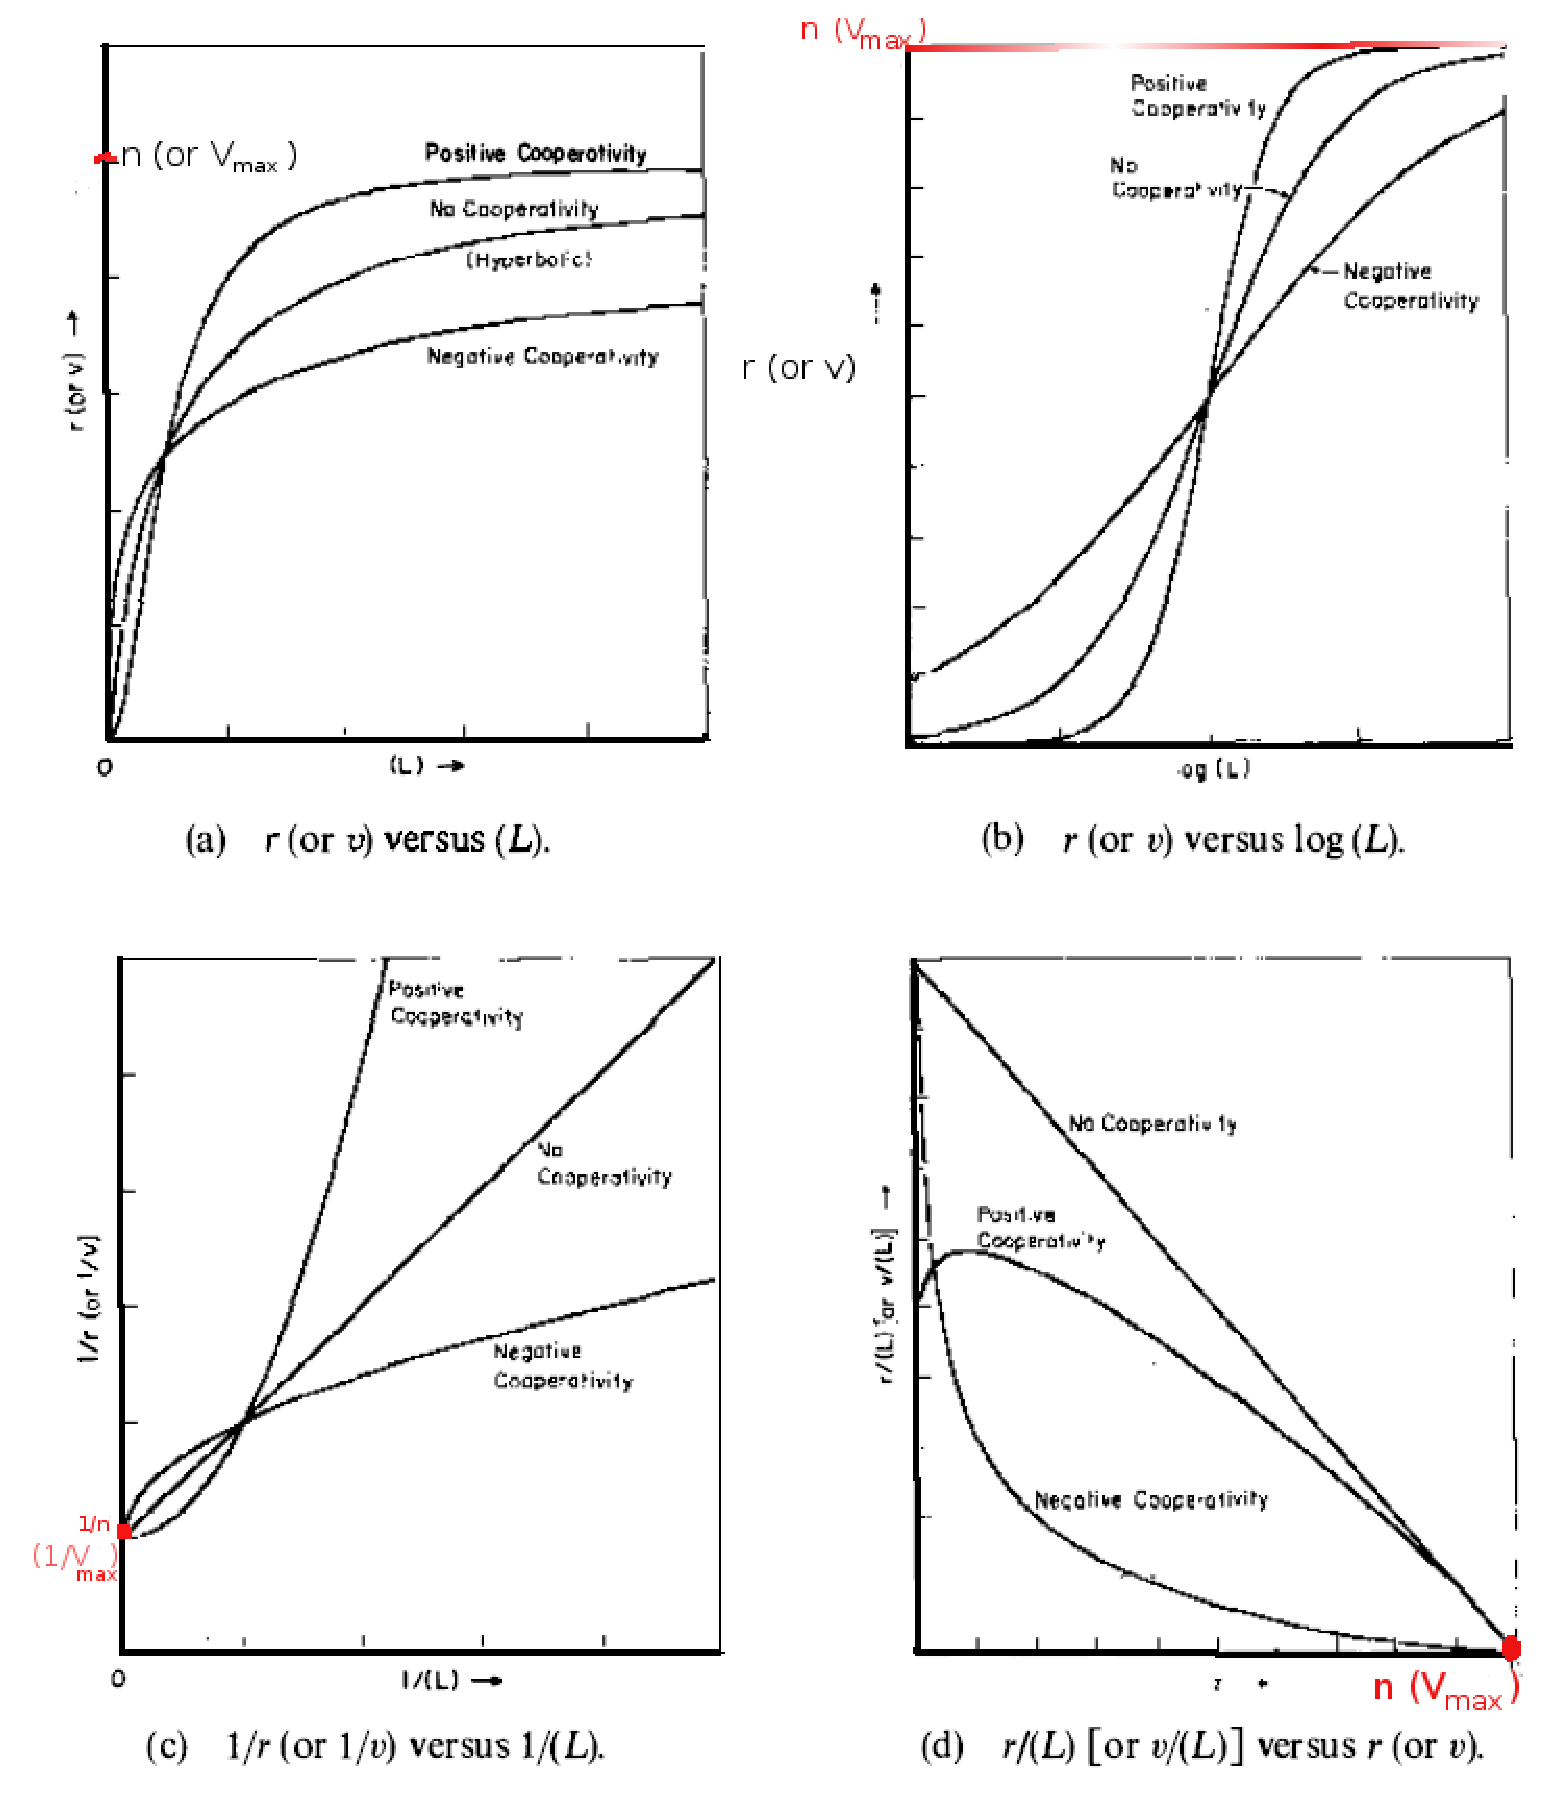
\includegraphics[height=11cm]{./images/enz_kin_curve.eps}}
\caption{Equilibrium binding and initial velocity of data. $r$ is the
  number of moles of ligand bound per mole of enzyme,$v$ is initial
  velocity of the enzymatic reaction, $n$ is the total number of
  ligand binding-site per enzyme molecule, $v_\max$ is the maximum velocity}
\label{fig:enz_kin}
\end{figure}

\begin{figure}[hbt]
 \centerline{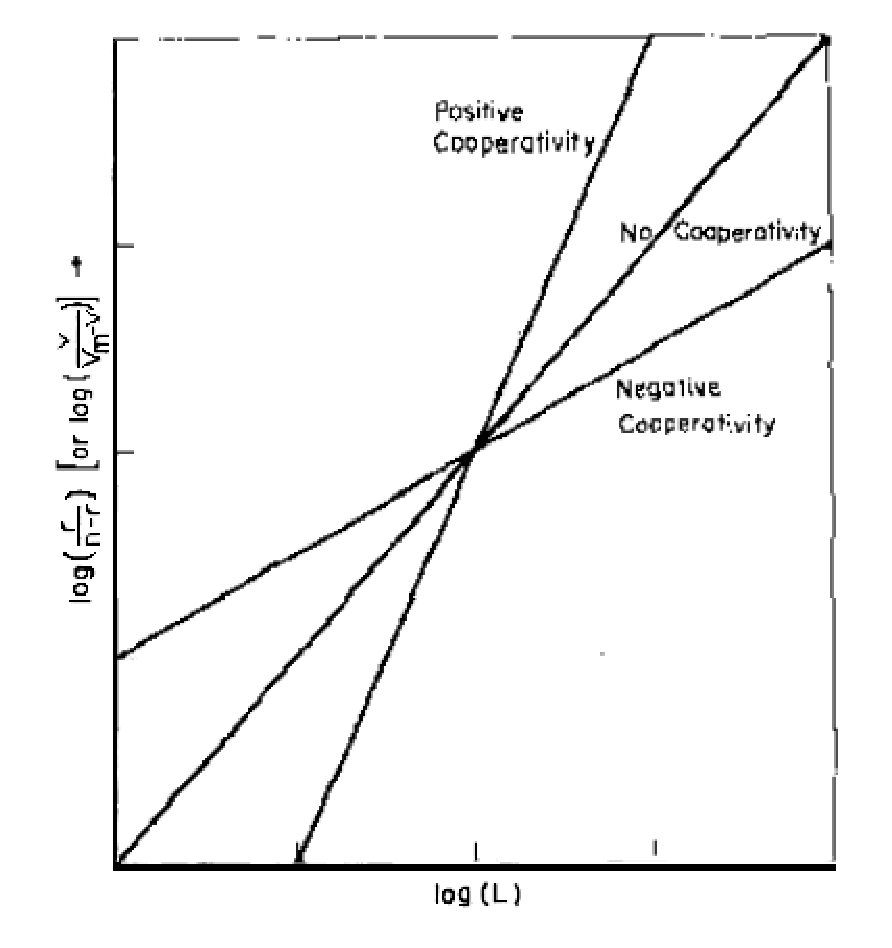
\includegraphics[height=8cm]{./images/enz_kin_2.eps}}
 \caption{Illustration of Hill plots. $r$ is the number of moles of
   ligand bound per mole of enzyme,$v$ is initial velocity of the
   enzymatic reaction, $n$ is the total number of ligand binding-site
   per enzyme molecule, $v_\max$ is the maximum velocity}
\label{fig:enz_kin_2}
\end{figure}

\subsection{Multiple catalytic binding sites - cooperative binding}
\label{sec:dissociation-curve}
\label{sec:cooperativity}

Typically, in a multiple-binding-site model, the binding of one
substrate can enhance/degrade the affinity of binding of subsequent
substrates. This is known as {\bf cooperativity}. 

Cooperativity, or concerted action, of multiple subunit proteins is a well
recognized phenomenon, the classic example being hemoglobin's increase in
affinity for additional oxygen molecules after one, two, or three have bound. 

In the previous sections, the velocity follows the simple hyperbolic curve,
Fig.~\ref{fig:rate_reaction}, Fig.~\ref{fig:Morrison_kin},
Fig.~\ref{fig:K_system}, Fig.~\ref{fig:enzyme_K_V}. However,
\textcolor{red}{many of the enzyme systems has the reaction velocity follow a
sigmoidal shape}. And it is cooperativity behavior that can produce such
sigmoidal shape.

{\bf Knowledge base}: Cooperative binding occurs in system with three
or more molecules when the binding of one molecule affects the binding
of others. This effect can be positive or negative. By positive, it
means that the binding of B to A will increase the affinity of A for
C. By negative, it means that the binding of B to A will decrease the
affinity of A for C. 

\subsection{-- Example}
\label{sec:example}

{\bf Example}\footnote{\url{http://www.ventworld.com/resources/oxydisso/dissoc.html}}:
Haemoglobin (Hb) is an intracellular protein that serves as the primary vehicle for transporting oxygen in
blood\footnote{Oxygen is also carried by (dissolved) in plasma, but in
  a much lesser degree}.
Hemoglobin is contained in erythrocytes (red blood cells).  Each Hb
molecule has a maximum capacity of carrying oxygen. The current
capacity of carrying oxygen  is dependent upon the specific
physiological condition. How much of that capacity at any time is 
called the {\it  oxyhaemoglobin saturation} ($Sa_{O_2}$), expressed in
percentage and is formulated as the ratio of the amount of oxygen
bound to the hemoglobin to the (maximum) oxygen carrying capacity of the
Hb. 

% Oxygen carrying capacity of the Hb is determined by the amount of Hb
% present in the blood.
\begin{equation}
  \label{eq:304}
  Sa_{O2} = \frac{\text{amount of oxygen bound to Hb}}{\text{amount
      of Hb}} 100\%
\end{equation}

% Depending upon the suitable conditions, oxygen bound to the Hb is
% released into the body tissue, or oxygen is observed from the tissue
% into the blood. Each Hb molecule has a capacity of carrying \ce{O2}
% molecules.

The amount of oxygen bound to Hb at any time is related, in large
part, to the {\bf partial pressure of oxygen} ($Pa_{O_2}$) in
blood. This value is high at lung and low at other body tissues. At
high $Pa_{O_2}$, oxygen are readily to bind to Hb; otherwise, HB cannot
maintain its full bound capacity of oxygen and thus oxygen are
released to tissue cells.

The behavior of oxygen transport by haemoglobin (Hb) at different
conditions of pH, \ce{CO2}, temperatures has been intensively studied
to increase the accuracy.  This is often represented as an
{\bf oxygen dissociation curve} (ODC) (or interactive oxyhemoglobin
dissociation curve) with x-axis is $Pa_{O_2}$ and y-axis is $Sa_{O_2}$, as
shown in Fig.~\ref{fig:SDC_plot}. 

\begin{figure}[hbt]
  \centerline{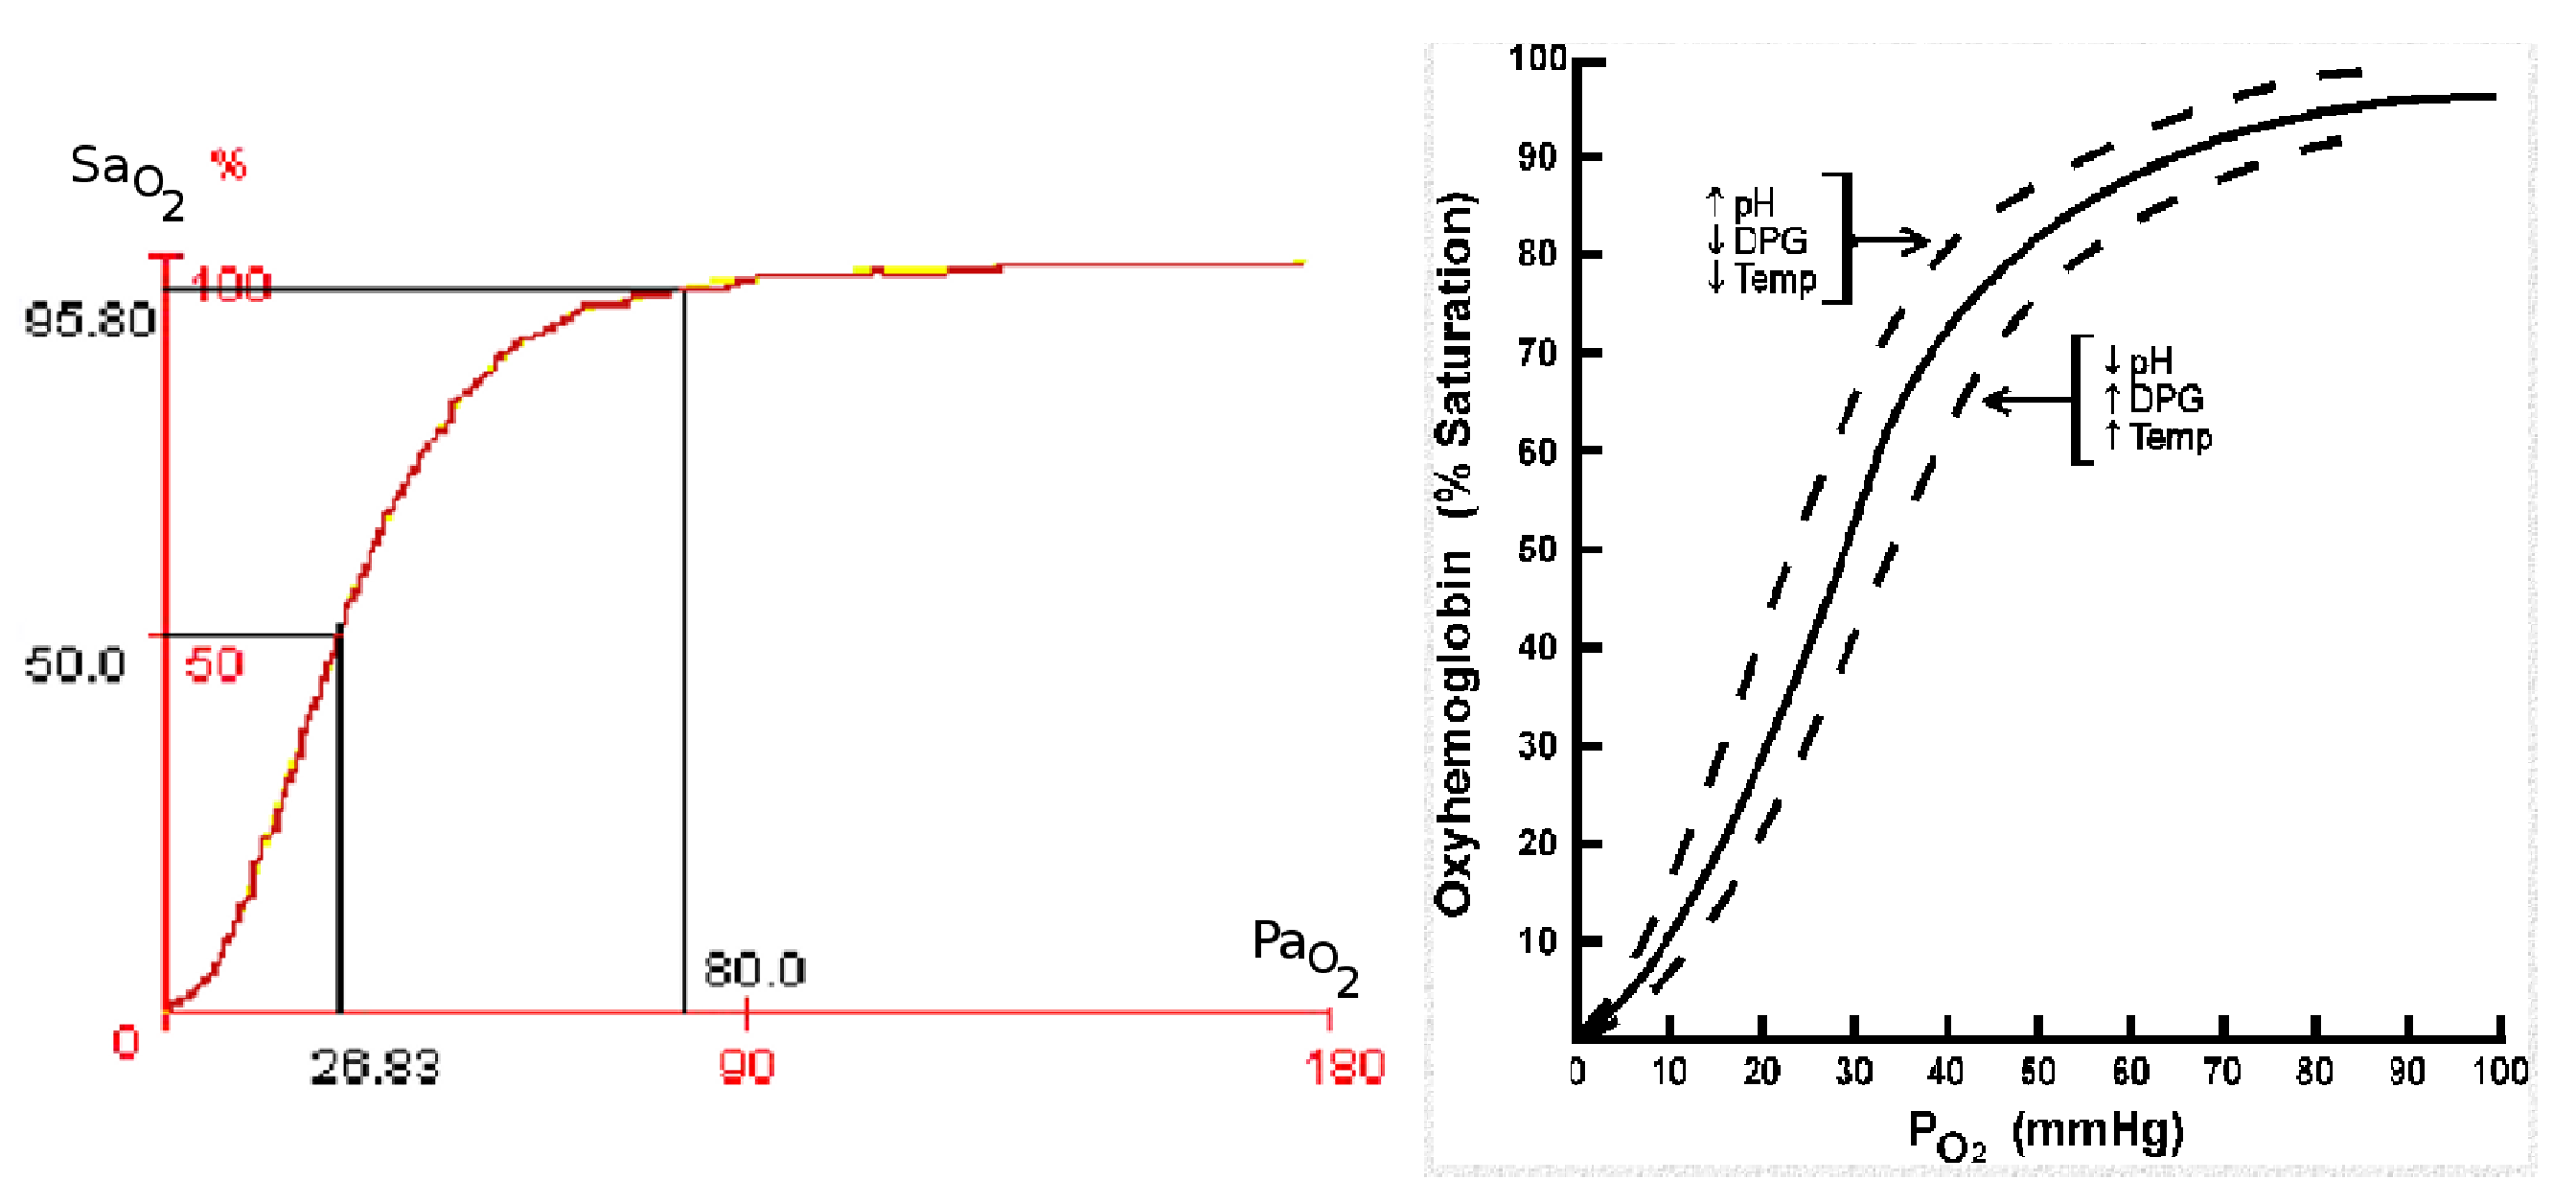
\includegraphics[height=5cm]{./images/PO2_SO2_plot.eps}}
  \caption{Standard ODC plot showing P50, and SO2 at PO2=80mmHg}
  \label{fig:SDC_plot}
\end{figure}

Commonly, the curve is plotted along with the $P_{50}$ value. This is
the value which tells the pressure at which SO2 is
50\%\footnote{\url{http://www.bio.davidson.edu/Courses/anphys/1999/Dickens/Oxygendissociation.htm}}.
The curve has a sigmoidal or S-shape. 

{\bf Why ODC is sigmoidal?}: Hb absorbs \ce{O2} rapidly in the range
20-40mmHg. At PO2 above 60 mmHg, the standard SDC curve is relatively
flat, i.e oxygen content does not change significantly even with large
increase of partial pressure of oxygen.  As partial pressure of oxygen
increase, the saturation of oxygen increase also, until a maximum
capacity can be reached. As this limit is reached, very little
additional binding occurs and the curve levels out as the haemoglobin
become saturated with oxygen.

% Thus, to get more oxygen to the tissues, either the oxygen have to
% dissolve more into the plasma, or the body then need more Hb.

One of the first person who derived the mathematical formula for this
relation is~\citep{hill1910pea}. Hill postulated that
cooperative binding occurs between Hb and \ce{CO2}. The aggregation
between haemoglobin and oxygen can occur at different levels, e.g.
\begin{equation}
  \label{eq:302}
  \begin{split}
    \ce{Hb + O2 <=>[k_1] HbO2} \\
    \ce{HbO + O2 <=>[k_2] HbO4} \\
    ... \\
    \ce{HbO_{n-2} + nO2 <=>[k_n] HbO_{2n}}
  \end{split}
\end{equation}
with $n$ is the ``number'' of molecules of oxygen to bind to a single
Hb molecule, $k_i$ are association constants (reaction
quotients, or Hill coefficient)~\citep{leow2007odc}. Using the law of mass actions, we have
\begin{equation}
  \label{eq:305}
  k_i = \frac{[\ce{HbO_{2i}]}}{[\ce{HbO_{2i-2}}][\ce{O2}]} = 
  \frac{[\ce{HbO_{2i}]}}{k_1k_2...k_{i-1}[\ce{Hb}][\ce{O2}]^{i}} 
\end{equation}
In essence, the net association constant for the overall reversible
process is
\begin{equation}
  \label{eq:306}
  K_n =k_1k_2...k_{n-1}k_n= \frac{[\ce{HbO_{2n}]}}{[\ce{Hb}][\ce{O2}]^{n}} 
\end{equation}
Under the assumption that all oxyhemoglobin at any point in time is
predominantly in the form of $\ce{HbO_{2n}}$, then using the law of
conservation of mass: 
\begin{equation}
  \label{eq:307}
  \begin{split}
    \text{total Hb} &= \text{total deoxygenated Hb + total
      oxyhemaglobin} \\
    &= [Hb] + [HbO_{2n}] \\
    &= [Hb] + K_n[Hb][\ce{O2}]^n
  \end{split}
\end{equation}

Then
\begin{equation}
  \label{eq:308}
  \begin{split}
    \ce{SaO2} &= \frac{\text{total oxyhemoglobin}}{\text{total Hb}} \\
    &= \frac{[\ce{HbO_{2n}}]}{ [Hb] + K_n[Hb][\ce{O2}]^n} \\
    &= \frac{K_n[\ce{O2}]^n}{ 1 + K_n[\ce{O2}]^n}
  \end{split}
\end{equation}
This is known as {\bf Hill equation} with a reasonable approximation
to Hb-oxygen data is $n\approx 2.6$. 

Adair \citep{adair1925odc} developed a 4-constant equation
({\bf Adair equation}) that's better fit the data. The four constants
related to the successive affinity constant of oxygen to the four heme
groups in Hb. Later, Pauling made the first attempt to give a
theoretical explanation for the changing affinity constants, i.e. to
the conformation of the proteins Hb (geometry of the 4 subunits).

Oxygen dissociation curve (ODC) have been attacked by many
researchers, yet there is no complete satisfying reason why the curve
has a form adapted to the needs of the organism, rather than the form
given by the simple laws of physics and chemistry.


When enzyme E is cooperative binding to substrate S to form \ce{ES_n},
the we have
\begin{equation}
  \label{eq:341}
  \begin{split}
    ES_n &= \frac{K_n[S]^n}{1+K_n[S]^n} \\
    &= \frac{[S]^n}{1/K_n+[S]^n} 
  \end{split}
\end{equation}

\subsection{-- Extreme Cooperativity (Hill equation)}

Consider an example when an enzyme has 2 binding sites
\begin{equation}
  \label{eq:269}
  \begin{split}
    \ce{S + E <=>[k_1][k_{-1}] C1 ->[k_2] E + P } \\
    \ce{C1 + S <=>[k_3][k_{-3}] C2 ->[k_4] C1 + P } 
  \end{split}
\end{equation}
The reaction velocity of the systems as determined by two slower
reactions, which is represented via $k_2, k_4$. Using assumption of
quasi-steady-equilibrium, we have $dc_1/dt=dc_2/dt=0$, then
\begin{equation}
  \label{eq:1372}
  \begin{split}
    c_1 = \frac{K_2e_0.s}{K_1K_2+K_2s+s^2} \\
    c_2 = \frac{e_0.s^2}{K_1K_2+K_2s+s^2}
  \end{split}
\end{equation}
with $K_1=\frac{k_{-1}+k_2}{k_1}$, $K_2=\frac{k_{-3}+k_4}{k_3}$. The
reaction velocity is defined as
\begin{equation}
  \label{eq:1373}
  v = k_2c_1 + k_4c_2 = \frac{(k_2K_2+k_4s)e_0.s}{K_1K_2+K_2s+s^2}
\end{equation}
\begin{enumerate}
\item Under the assumptions that the two active sites are independent
  and identical, then $k_1=2k_3$, and $k_{-3}=2k_{-1}$ and
  $2k_2=k_4$. The factors of 2 is chosen because there are two
  identical binding sites, which doubling the amount of
  reactions. Then eq.~\eqref{eq:1373} becomes
\begin{equation}
  \label{eq:1374}
  v = 2\frac{k_2e_0.s}{K+s}=\frac{k_4e_0.s}{K+s}
\end{equation}
with $K=\frac{k_{-1}+k_2}{k_3}$.


\item Under the assumption that the binding of the first substrate is
  low, yet the binding of the second one is fast (thanks to the
  binding of the first one). So, we let $k_3\rightarrow\infty$,
  $k_1\rightarrow 0$ while keeping $k_1k_3=$constant. Then,
  $K_2\rightarrow 0$, and $K_1\rightarrow \infty$ while
  $K_1K_2=$constant. In this case, eq.~\eqref{eq:1373} becomes
  \begin{equation}
    \label{eq:1375}
    v = v_\max \frac{s^2}{K_m^2+s^2}
  \end{equation}
with $K_m^2=K_1K_2$.


In general, if there are $n$ binding sites, with the assumptions
$K_n\rightarrow 0$, $K_1\rightarrow\infty$ and $K_1K_n=$ constant,
then 
\begin{equation}
  \label{eq:1376}
  v = v_\max \frac{s^n}{K_m^n+s^n}
\end{equation}
with $K_m^n=\pi^n_{i=1}K_i$. This is known as {\bf Hill equations}.

NOTE: $n, K_m$, and $v_\max$ are determined from experimental data,
using {\bf Hill plot} (Fig.~\ref{fig:enz_kin_2}) which plot
$\ln(v/(v_\max-v)$ against $\ln s$.
\begin{equation}
  \label{eq:1377}
  n\ln s = n\ln K_m + \ln\left(\frac{v}{v_\max-v}\right)
\end{equation}
In practice, for the best fit, $n$ can be a non-integer.  

\end{enumerate}

\subsection{-- Negative cooperativity}
\label{sec:negat-coop}

Negative cooperativity decrease the velocity, similar to V-system
(Sect.~\ref{sec:competitive-two-site}). This can be modelled by
decreasing $k_3$, Fig.~\ref{fig:cooperativity}.
Using quasi-steady-state approximation, the velocity of the reaction
for an enzyme with allosteric inhibitor is
\begin{equation}
  \label{eq:1390}
  v = v_\max\frac{K_3}{i+K_3}
  \left( \frac{s(k_{-1}+k_3i+k_1s+k_{-3})}{k_1(s+K_1)^2+(s+K_1)(k_3i+k_{-3}+k_2)+k_2k_{-3}/k_1}\right)
\end{equation}
where $K_3=k_{-3}/k_3$ and $K_1=k_{-1}/k_1$.

\begin{figure}[hbt]
  \centerline{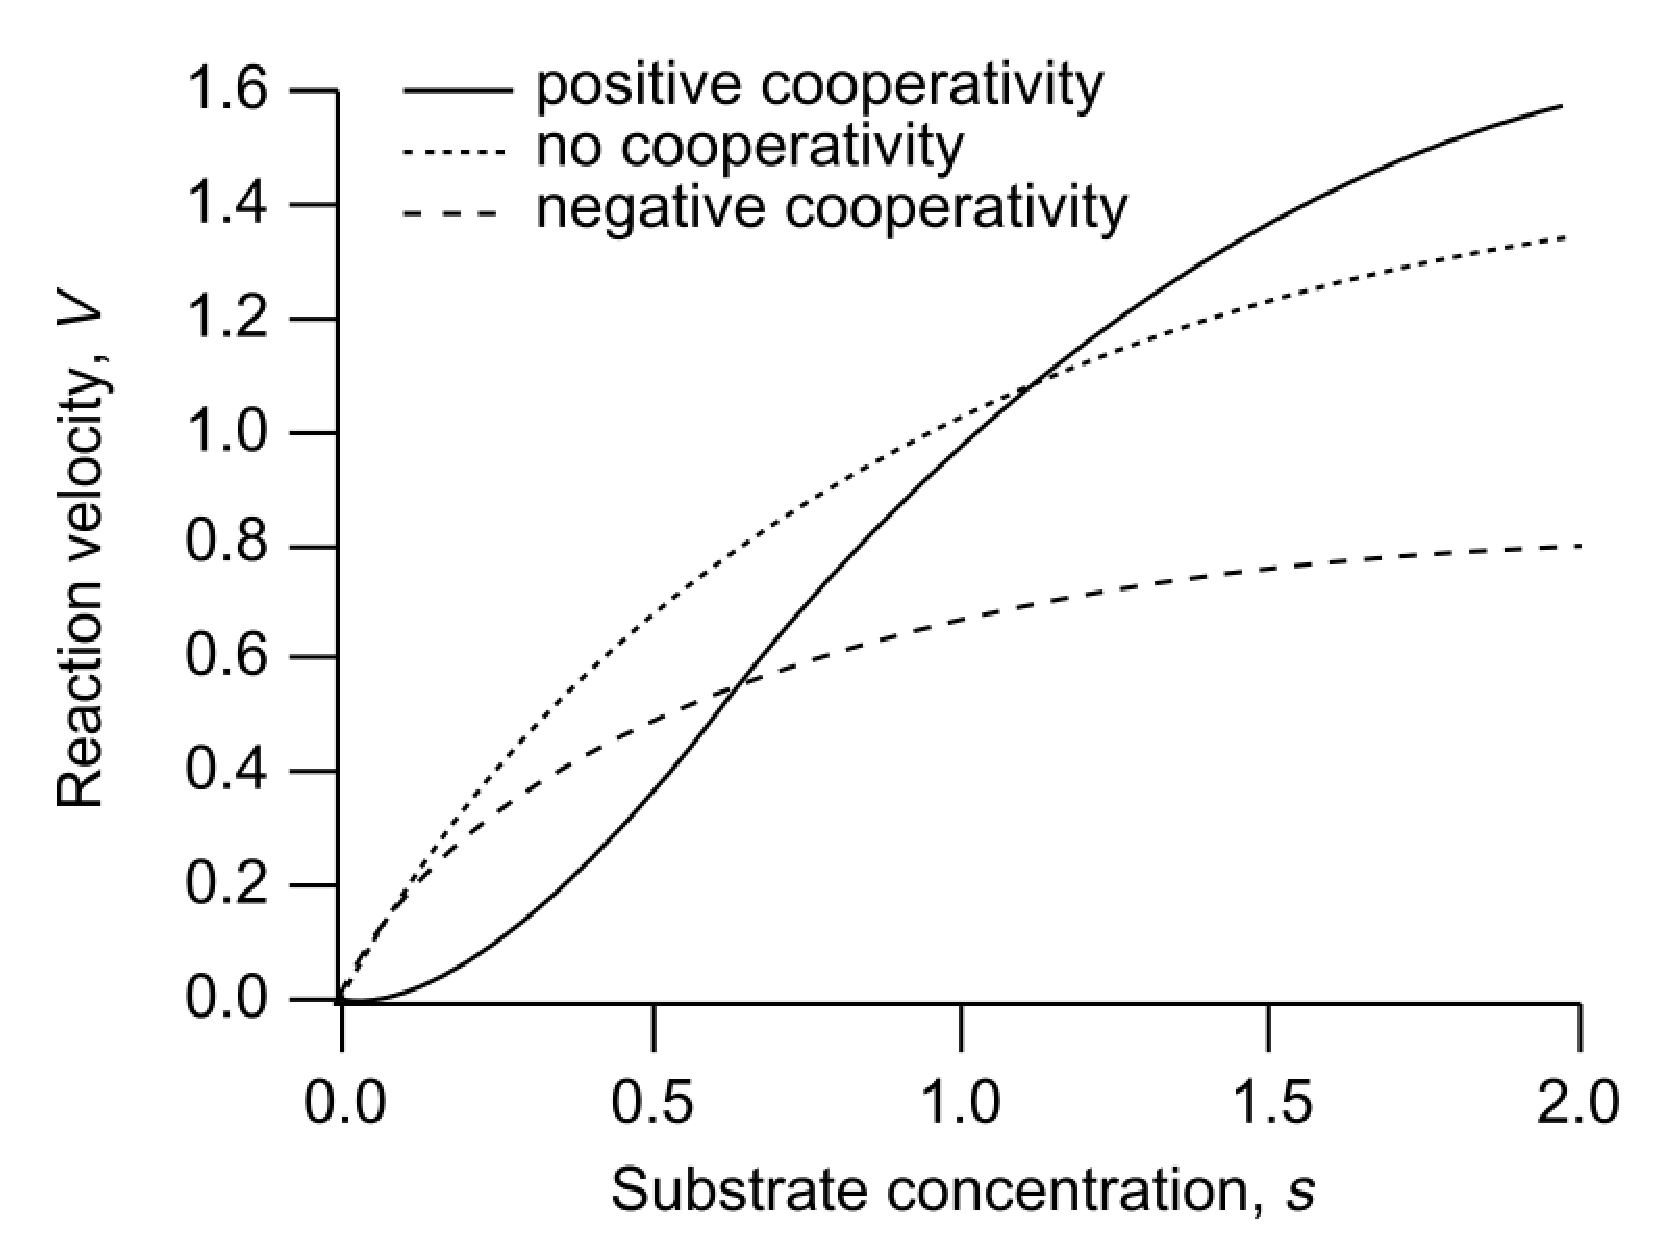
\includegraphics[height=5cm,
    angle=0]{./images/cooperativity.eps}}
  \caption{positive cooperativity ($K_1=1000, K_2=0.001$), independent
    binding ($K_1=0.5,K_2=2$), negative cooperativity
    ($K_1=0.5,K_2=100$). The other parameters were chosen as
    $e_0=1,k_2=1,k_4=2$ (unit arbitrary)}
\label{fig:cooperativity}
\end{figure}

\subsection{-- Cooperativity factor}
\label{sec:coop-fact}

Cooperativity factor describes the level of cooperativity that arise
when the binding of one molecule affect the binding of
ano1ther. Suppose that A is an enzyme, B and C are two
substrates. Then, the dissociation constant between A and C is
$K_{D(AC)}$ and that between A and B is $K_{D(AB)}$. When $B$ bind to
A first, it affect the dissociation constant between A and C by a
factor $\alpha$. Alternatively, when $C$ bind to A first, it affect
the dissociation constant between A and B a factor $\beta$. 

Both $\alpha$ and $\beta$ are called cooperativity factors. They are
not Hill coefficient, yet both types are used to describe
cooperativity. When $\alpha$ (or $\beta$) is greater than 1, a system
has negative cooperativity. When it is equal to 1, a system lack
cooperativity. When it is smaller than 1, a system has positive
cooperativity. 
\begin{equation}
  \label{eq:342}
  \begin{split}
    &A + B \;\;\; \ce{<=>[K_{D(AB)}]} AB \\
    &+ \;\;\;\;\;\;\;\;\;\;\;\;\;\;\;\;\;\;\;\;\;\;\;  + \\
    &C\;\;\;\;\;\;\;\;\;\;\;\;\;\;\;\;\;\;\;\;\;\;\;\;\;\;  C \\
    K_{D(AC)}&\upharpoonleft\downharpoonright  \;\;\;\;\;\;\;\;\;\;\;\;\;\;\;\;\;\;\;\;\;\;    \upharpoonleft\downharpoonright\alpha K_{D(AC)} \\
    &AC + B \ce{<=>[\beta K_{D(AB)}]} ABC
  \end{split}
\end{equation}

\subsection{-- Mechanistic models of cooperativity}
\label{sec:mech-models-coop}

There were 2 different types of ligands: regulatory effectors and substrates.
They bind to the target protein at topographically distinct sites; yet mutually
influence each other through a reversible conformational change. This concept of
indirect or ``allosteric'' interactions was different from the classical
explanation of enzyme inhibition through steric hindrance at a common binding
site. The second issue is the cooperative (homotropic) interactions of some
identical ligands. A mechanistic explanation for the cooperativity binding model
was proposed by~\citep{monod1965nat}, known as {\bf Monod-Wyman-Changeux model}
(MWC). A literature review of other models is given by~\citep{dixon1979,
changeux2005}.


Assumptions being used by Monod-Wyman-Changeux model
\begin{enumerate}
  \item The regulatory proteins have a quaternary structure with identical
  subunits with symmetry properties. An enzyme (i.e. cooperative proteins) is
  composed of several identical reacting units, called {\bf promoters}, that occupy
  equivalent positions within the protein.
  
\item Each promoter contains one binding site for each ligand

\item The binding sites within each enzyme are equivalent

\item If the binding of a ligand to one promoter and induce the
  conformational change in that promoter; it also induce identical
  conformational change in all other promoters.
  
\item The enzyme has 2 conformational states, denoted by R and T,
  which differ in their binding affinity to ligands. T = low-affinity
  low-activity, R = high-affinity, high-activity state.
\end{enumerate}
The conformational R-T equilibrium is an intrinsic property of the allosteric
oligomers accessible in the absence of ligand. Here, ligands control protein
functin by altering a pre-existing equilibrium between high (R) and low (T)
reactive conformations.  Due to its simplicity, the postulated 2-state
``concerted'' transition has been a debated issue. There have been other
alternative sequential model with multiple conformations, each with different
numbers of ligand molecules bound \citep{viappiani2004}. 

{\bf Example}: An enzyme has 2 binding sites, i.e. 2 promoters. So,
for each conformational state, there can be 0, 1 or 2 ligands
binding. Totally, there are 6 states: $R_i$ (i=0,1,2) and $T_i$
(i=0,1,2). If we assume $R_1$ cannot convert directly to $T_1$ and
similar to $R_2$ and $T_2$, the schematic diagram for the kinetics of
the enzyme is given in Fig.~\ref{fig:MWC_model}.

\begin{figure}[hbt]
  \centerline{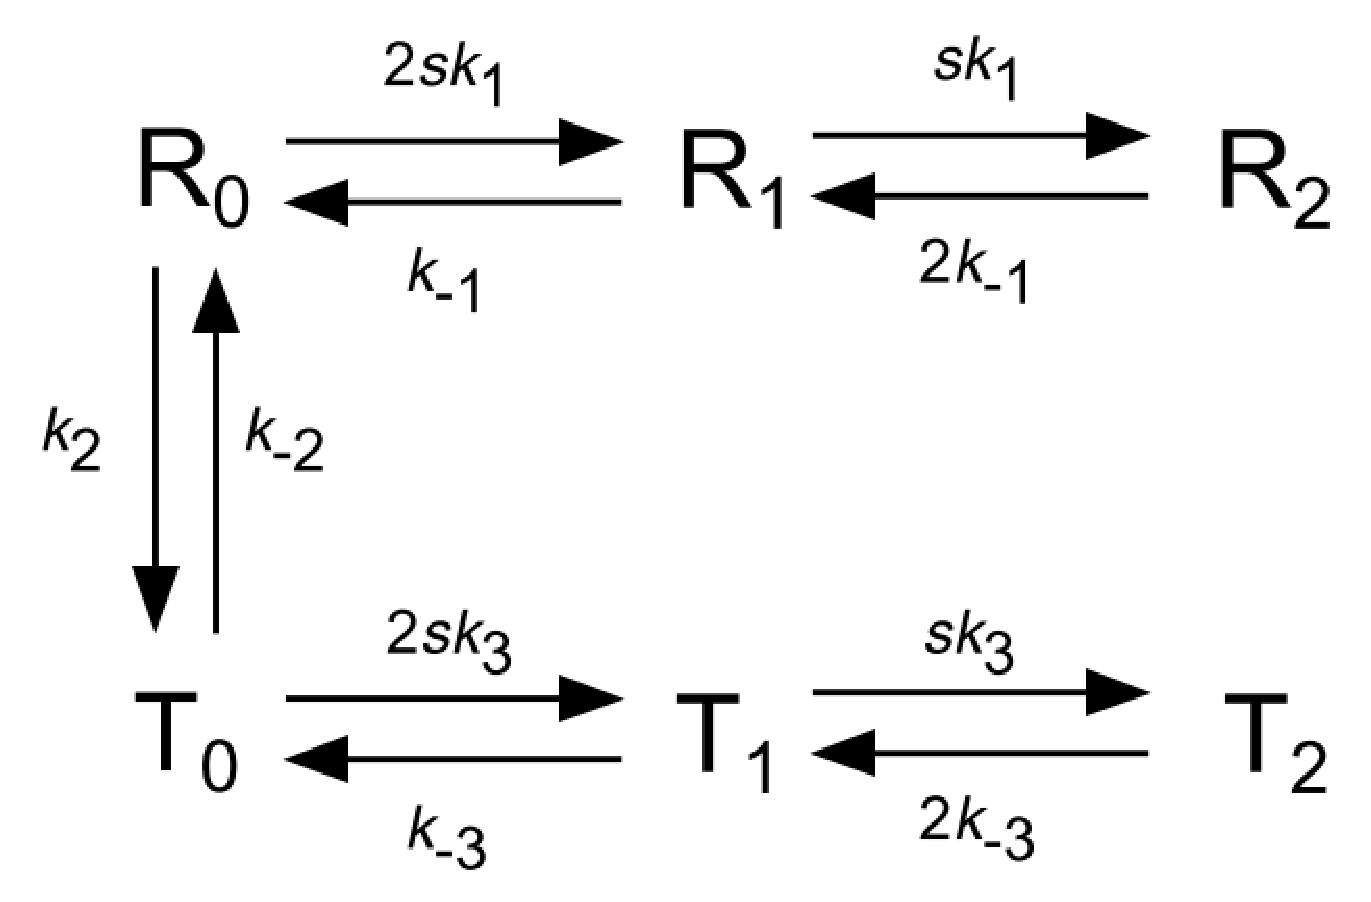
\includegraphics[height=5cm,
    angle=0]{./images/MWC_model.eps}}
\caption{An example of Monod-Wyman-Changeux model}
\label{fig:MWC_model}
\end{figure}
To estimate the rate constants, we assume that all reactions are in
equilibrium. Let denotes $r_i$ and $t_i$ are constants of chemical
species in the corresponding state. Using $s$ as the concentration of
the substrate, then the fraction Y of occupied sites (saturation
function) is
\begin{equation}
  \label{eq:1386}
  Y = \frac{}{}
\end{equation}

If there are $n$ binding sites, then 
\begin{equation}
  \label{eq:1387}
  Y = \frac{sK_1^{-1}(1+sK_1^{-1})^{(n-1)} + K_2^{-1}
  \left[  sK_3^{-1}(1+sK_3^{-1})^{(n-1)}\right]}{(1+sK_1^{-1})^n+K_2^{-1}(1+sK_3^{-1})^n}
\end{equation}
\textcolor{red}{Y is a sigmoidal function of $s$}.

Special cases:
\begin{enumerate}
\item $K_2=\infty$ (i.e. only the conformation R exists), then
  \begin{equation}
    \label{eq:1388}
    Y = \frac{s}{s+K_1}
  \end{equation}
\item $K_3=\infty$ (i.e. the substrate cannot bind directly to the T
  conformation)
  \begin{equation}
    \label{eq:1389}
    Y = \frac{sK_1^{-1}(1+sK_1^{-1})}{(1+sK_1^{-1})^2+K_2^{-1}}
  \end{equation}
\end{enumerate}




\section{Stochastic model of enzyme kinetics}
\label{sec:stoch-model-enzyme}


\begin{framed}
  With stochastic behavior, the reaction rate can be considered as
  the product of the number of collisions per unit of time between $A$
  and $R$ and the probability that a collision can produce $C$, or in
  other words, the energy released from the collision is high enough
  to pass the reaction energy. Then, only the number of collisions per
  unit of time is the deterministic part; and a random number, that
  determine the completion of the reaction is the stochastic part. 

  The unit of the {\it rate constant} depending on the type of the
  reaction; e.g. unimolecular or bimolecular or .... In addition, its
  value also depends on the geometrical shapes and sizes of the
  reactant molecules, as well as the temperatures of the mixture.
\end{framed}

A prior probability is assigned 
\begin{itemize}
\item for the two molecules S and E to collide and form the complex
\item for a complex to be broken down to E and P
\item for a complex to be separate into E and S.
\end{itemize}

Thus, the framework for the mode is given
\begin{itemize}
\item [Axiom 1] Given at a time $t$ (after mixing S and E), the
  mixture has $n_1$ molecules (per constant volume) of free enzyme E
  and $n_2$ molecules of substrate S. So, the probability for forming
  a new complex ES in the time interval $(t,t+\Delta t)$ is
  \begin{eqnarray}
    \label{eq:2}
    n_1n_2[\mu_1.\Delta t + O(\Delta t)]
  \end{eqnarray}
  with $\mu_1.\Delta t + O(\Delta t)$ is the probability for each pair
  to combine, $\mu_1$ is the mean (or the rate transition) 
\item [Axiom 2] Given at a time $t$ (after mixing S and E), the
  mixture has $n_3$ molecules (per constant volume) of free complex
  ES. So, the probability for dissociating back to E and S in the time
  interval $(t,t+\Delta t)$ is
  \begin{eqnarray}
    \label{eq:2}
    n_3[\mu_2.\Delta t + O(\Delta t)]
  \end{eqnarray}
  with $\mu_2.\Delta t + O(\Delta t)$ is the probability for each
  complex molecule to dissociate, $\mu_2$ is the mean (or the rate
  transition) 
\item [Axiom 3] Given at a time $t$ (after mixing S and E), the
  mixture has $n_3$ molecules (per constant volume) of free complex
  ES. So, the probability for the complex to pass the energy barrier
  to make the product P in the time interval $(t,t+\Delta t)$ is
  \begin{eqnarray}
    \label{eq:2}
    n_3[\mu_3.\Delta t + O(\Delta t)]
  \end{eqnarray}
  with $\mu_3.\Delta t + O(\Delta t)$ is the probability for each
  complex molecule to pass the energy barrier, $\mu_3$ is the mean (or
  the rate transition).
\end{itemize}
and $O(\Delta t)$ represents the fluctuations, or the randomness at
each time step.

For the three above conditions to satisfy, other assumptions involves:
\begin{enumerate}
\item The individual molecular events are all statistically
  independent, i.e. the probabilities for joint occurrences of all
  kinds are determinable as the products of the probabilities of the
  individual component events.
\item Initially, the number of substrate molecules is far in excess of
  the number of enzyme molecules.
\item Environmental physical parameters (T, p, pH) are assumed
  constant for the entire interval, rendering the rate transition
  $\mu_1, \mu_2, \mu_3$ constant.
\end{enumerate}
The rate constant $k_i$ in classical enzyme kinetics is mapped to the
probability parameter $\mu_i$ (for more detail, read Chap.10 (sec 5)
of the Computational Biology book). In the context of Markov-Chain
Theory, it is an ``intensity number'' i.e. an element of the
``Q-matrix'' that determines the transition probabilities of the
process from one concentration state to another.
\textcolor{red}{One can say that
  {\it the stochastic model agrees ``on the average'' with the
    deterministic one; or the former one is consistent in the mean''
    with the latter}}~\citep{bartholomay1962errt}.

In this problem, there are totally 4 quantities, $n_i$. Suppose $n_4$
is the number of product molecules at time $t$, then $n_{i0}$ (i=1..4)
is the number of molecules for each species at time $t=0$, with
$n_{30}=n_{40}=0$. Based on the law of conservation, we have
\begin{equation}
  \label{eq:4}
  \begin{split}
    n_1 &= n_{10} - n_3 \\
    n_4 &= n_{20} - (n_2+n_3)
  \end{split}
\end{equation}
Eventually, the problem turns into two canonical variables $n_2,n_3$.
The probability, at time $t$, in the mixture there are $n_2,n_3$
molecules of substrate S and complex [ES] is denoted as
$p(n_2,n_3,t)$.  In the small time step, it is assumed that only one
reactive event to take place, i.e. $n_i$ either doesn't change,
increase one or decrease one.
(\textcolor{red}{this is the basic idea to formulate the Markov-Chain
  Monte-Carlo simulation using Q-matrix}).
A good explanation for this assumption can be referenced in
Bartholomay (1961)~\citep{bartholomay1962errt}.  If $n_2$ and $n_3$ are
independent, there would be $3\times 3=9$ ways. However, from
eq.~\eqref{eq:4}, they are interrelated. So, given the value of the
current time is $n_2,n_3$, for the next time step, there are only 4
mutually exclusive possible cases:
\begin{enumerate}
\item [$E_1$] no change in the next time step: $n_2,n_3$
\item [$E_2$] substrate doesn't change, complex change one (make product):
  $n_2,n_3-1$
\item [$E_3$] substrate reduce one (to form complex), complex increase one:
  $n_2-1,n_3+1$
\item [$E_4$] substrate increase one, complex decreases one (dissociate):
  $n_2+1,n_3-1$
\end{enumerate}
We then set up 4 difference equation of the form
\begin{eqnarray*}
 E_i =  p(n'_2,n'_3,t+\Delta t) - p(n_2,n_3,t)
\end{eqnarray*}
with $\sum E_i = 1$. So, in the stochastic modelling, if the random
follow the uniform distribution, to know the next state of the
mixture, we generate a random number X, e.g. using uniform
distribution and see which range that X fall into. This is exactly the
same as Markov-Chain Monte-Carlo simulation. 

\section{Tools for enzyme kinetics}
\label{sec:tools-enzyme-kinet}


\subsection{VisualEnzymics}
\label{sec:visualenzymics}

Visual Enzymics is a statistical analysis for enzyme kinetics. It
supports 5 types of enzyme kinetic data and 70 model equations
\footnote{\url{http://www.softzymics.com/models.htm}}.


% \section{Enzymatic reation-rate theory}
% \label{sec:enzym-reat-rate}

% Thus, at the equilibrium concentration, the concentration of A is
% \begin{eqnarray*}
%   A_0\mu_1\mu_2/(\mu_1+\mu_2)^2
% \end{eqnarray*}

